% Project report for Distributed Database System
% IEEE two-column format
\documentclass[10pt,conference]{IEEEtran}
\usepackage{times}
\usepackage{graphicx}
\usepackage{amsmath}
\usepackage{amssymb}
\usepackage{booktabs}
\usepackage{url}
\usepackage{cite}
\usepackage{caption}
\usepackage{subcaption}
\usepackage{color}
\usepackage{listings}
\usepackage{xcolor}
\usepackage{float}
\usepackage{tikz}
\usetikzlibrary{shapes,arrows,positioning,fit,backgrounds,calc,arrows.meta}

% TikZ styles for UML diagrams
\tikzstyle{component} = [rectangle, draw, fill=blue!10, text width=2.2cm, text centered, minimum height=1cm, font=\footnotesize]
\tikzstyle{database} = [cylinder, draw, fill=orange!20, shape border rotate=90, aspect=0.25, minimum height=1cm, minimum width=1.2cm, font=\footnotesize]
\tikzstyle{arrow} = [->, >=stealth, thick]
\tikzstyle{dashedarrow} = [->, >=stealth, dashed]
\tikzstyle{state} = [rectangle, rounded corners, draw, fill=green!10, text width=2cm, text centered, minimum height=0.8cm, font=\footnotesize]
\tikzstyle{actor} = [rectangle, draw, minimum width=0.8cm, minimum height=2cm]
\tikzstyle{lifeline} = [dashed, gray]
\tikzstyle{activation} = [rectangle, draw, fill=white, minimum width=0.3cm]
\tikzstyle{message} = [->, >=stealth]

% Code listing style
\lstset{
    basicstyle=\ttfamily\footnotesize,
    breaklines=true,
    frame=single,
    language=Python,
    keywordstyle=\color{blue},
    commentstyle=\color{gray},
    stringstyle=\color{red}
}

	\title{Distributed Database System with Logical Timestamps, Adaptive Quorums, and Performance-Aware Failover}

\author{
\IEEEauthorblockN{Keyaba Gohil\IEEEauthorrefmark{1}, Jayateerth Kamatgi\IEEEauthorrefmark{2}, and Satheesh Kumar G R\IEEEauthorrefmark{3}}
\IEEEauthorblockA{Department of Computer Science\\
San Jos\'e State University\\
\IEEEauthorrefmark{1}Email: keyaba.gohil@sjsu.edu\\
\IEEEauthorrefmark{2}Email: jayateerth.kamatgi@sjsu.edu\\
\IEEEauthorrefmark{3}Email: satheeshkumar.geetharavi@sjsu.edu}
}

\begin{document}

\maketitle

\begin{abstract}
This report presents the design, implementation, and evaluation of a distributed MySQL database system that addresses key challenges in distributed systems: consistency, fault tolerance, and performance optimization. Modern distributed databases must balance competing requirements: strong consistency for correctness, high availability for user experience, and low latency for performance. Our system implements three core algorithms drawn from recent research: (1) Timestamp as a Service for globally ordered writes without centralized coordination, enabling total ordering of operations while eliminating single points of failure; (2) Cabinet algorithm for adaptive quorum-based replication that dynamically selects the fastest and healthiest replicas, reducing write latency by up to 40\% compared to static configurations; and (3) SEER algorithm for performance-aware leader election during master failures, selecting new leaders based on latency, stability, and replication lag rather than arbitrary criteria.

The system is built using Docker containers with a FastAPI-based coordinator, four MySQL 8.0 instances (one master and three replicas), and dedicated microservices for metrics collection, quorum selection, and leader election. We provide tunable consistency levels (ONE, QUORUM, ALL) that allow applications to trade off between latency and durability based on their specific requirements. Our evaluation demonstrates that the adaptive approach reduces average write latency from 67ms (ALL) to 35ms (QUORUM with Cabinet), while maintaining strong consistency guarantees through quorum intersection. The system successfully handles master failures with automatic promotion of the best-performing replica, completing failover in 6-8 seconds with minimal data loss. Our implementation serves as both an educational tool for understanding distributed systems concepts and a foundation for production-grade distributed database research.
\end{abstract}

\begin{IEEEkeywords}
distributed databases, quorum replication, leader election, timestamps, consistency, fault tolerance, MySQL, Docker
\end{IEEEkeywords}

%==============================================================================
\section{Problem Description, Goals, and Motivation}
%==============================================================================

When working with distributed databases, you typically want both consistency and availability even when things go wrong-for example, when the master database crashes or a replica falls behind. In practice, many real-world systems either rely on slow, manual failover scripts or use centralized coordination points that become bottlenecks and single points of failure. The challenge of building reliable distributed storage has been studied extensively since the early days of distributed computing, yet production systems continue to struggle with the fundamental tension between consistency, availability, and partition tolerance famously articulated by the CAP theorem \cite{cap}.

Commercial offerings such as AWS RDS illustrate this tension. A standard deployment runs with a single master and a set of read replicas. Writes only go to the master, and replication to replicas is asynchronous. If the master crashes, failover can take a noticeable amount of time, and there is no strict guarantee that replicas are fully up to date when applications read from them. Google Cloud SQL, Azure Database for MySQL, and similar managed services face analogous constraints. While they offer convenience and operational simplicity, they abstract away critical decisions about consistency semantics, failover behavior, and replica selection, leaving developers with limited visibility into how their data is being managed.

The problem becomes more acute as applications scale. Consider an e-commerce platform processing hundreds of transactions per second. A master failure during peak traffic can result in lost revenue, frustrated users, and potential data inconsistencies if the failover process is not carefully orchestrated. Similarly, a financial services application that reads stale data from a lagging replica might display incorrect account balances, leading to compliance violations or customer disputes. These are not hypothetical scenarios; they represent real challenges faced by engineering teams at companies of all sizes.

Our goal in this project is to design and implement a distributed MySQL-based system that does better along three axes: (1) it should \emph{handle failures automatically} without long outages, (2) it should \emph{preserve strong consistency guarantees} for writes, and (3) it should \emph{avoid centralized bottlenecks} wherever possible. Instead of building a key-value store from scratch, we deliberately chose a familiar relational database (MySQL) so that our system feels realistic and could, in principle, back a real application. We then identified concrete pain points observed in practice-slow failover, opaque replication status, and lack of tunable consistency-and used them as design drivers.

Beyond these functional goals, we also aim to create an educational artifact that makes distributed systems concepts tangible. Students and practitioners often learn about consensus, replication, and leader election in the abstract, without seeing how these ideas manifest in working code. By implementing Timestamp as a Service, Cabinet, and SEER as separate microservices with clear APIs, we provide a hands-on laboratory where each algorithm can be studied, modified, and benchmarked independently.

More formally, we want to provide an experience similar to a managed relational database service but with the knobs and visibility of a research prototype. Application developers should be able to issue familiar SQL queries without worrying about which physical node is currently the master, which replicas are lagging, or how leader election operates internally. At the same time, system designers should be able to introspect the internal metrics, algorithms, and decision logic to understand why a particular replica was chosen or why a failover event happened at a certain time.

To meet these goals, we use MySQL as the storage engine but layer it with three key ideas drawn from recent research:
\begin{itemize}
    \item \textbf{Logical timestamps} to keep writes in globally consistent order without a centralized timestamp oracle. By distributing timestamp generation across multiple servers with non-overlapping sequences, we eliminate a common single point of failure while preserving the total ordering property essential for serializability.
    \item \textbf{Adaptive quorum selection (Cabinet)} that favors faster, more up-to-date replicas. Rather than treating all replicas as interchangeable, Cabinet weights them by observed latency and replication lag, allowing the system to consistently route writes through the healthiest subset of the cluster.
    \item \textbf{Performance-aware leader election (SEER)} that picks the most stable and responsive replica if the master fails. Traditional leader election algorithms choose leaders based on node IDs or random selection; SEER instead uses historical performance metrics-latency, uptime, and crash frequency-to select a leader that is likely to perform well in the master role.
\end{itemize}

Together, these mechanisms give us a system that handles failure better, responds faster, and still maintains consistency guarantees. The combination is greater than the sum of its parts: timestamps provide ordering, Cabinet ensures writes go to healthy replicas, and SEER ensures that failover promotes the right node. The rest of this report expands on the problem, the related work, our methodology and system architecture, and a detailed evaluation of the resulting prototype.

\subsection{Problem Statement Summary}

To summarize, the core problems we address are:
\begin{enumerate}
    \item \textbf{Slow and manual failover}: Existing systems often require human intervention or lengthy automated scripts to recover from master failures, resulting in extended downtime.
    \item \textbf{Suboptimal replica selection}: Fixed quorum configurations do not account for runtime performance variations, leading to unnecessarily high write latencies.
    \item \textbf{Centralized timestamp bottlenecks}: A single timestamp oracle becomes both a performance bottleneck and a single point of failure.
    \item \textbf{Lack of tunable consistency}: Many systems offer only a single consistency model, forcing developers to accept trade-offs that may not match their application's requirements.
    \item \textbf{Limited observability}: Developers cannot easily understand why the system made particular routing or failover decisions, making debugging and optimization difficult.
\end{enumerate}

Our distributed database prototype addresses each of these problems with concrete, measurable mechanisms that we describe and evaluate in the following sections.

%==============================================================================
\section{Project Goals and Distributed System Challenges}
%==============================================================================

Our project is guided by two sets of objectives: concrete project goals specific to our system, and general distributed system challenges drawn from the course. These objectives shaped every design decision, from the choice of MySQL as the storage layer to the microservice architecture that separates concerns into independently deployable components.

\subsection{Project Goals}

At a high level, the project goals are:
\begin{itemize}
    \item \textbf{Single Logical Endpoint}: Provide a single logical SQL endpoint that hides the complexity of multiple MySQL instances and microservices. Clients should interact with the system using familiar SQL syntax without needing to understand the underlying distributed infrastructure.
    
    \item \textbf{Three Distributed Algorithms}: Implement at least three distributed algorithms (timestamps, quorum-based replication, and leader election) in a realistic setting. Each algorithm should be isolated in its own microservice with clear APIs, enabling independent study and modification.
    
    \item \textbf{Automatic Failure Handling}: Demonstrate automatic handling of server failures without manual intervention. The system should detect failures within seconds, elect new leaders when necessary, and continue serving requests with minimal disruption.
    
    \item \textbf{Tunable Consistency}: Expose tunable consistency and performance trade-offs that can be observed in experiments. Users should be able to choose between latency (ONE), balanced (QUORUM), and durability (ALL) modes based on their application requirements.
    
    \item \textbf{Educational Value}: Create a system that is both functional and educational. The codebase should be readable, well-documented, and structured to help students understand distributed systems concepts through working code.
\end{itemize}

\subsection{Mapping Goals to Implementation}

Table~\ref{tab:goals-mapping} shows how each project goal maps to specific implementation components.

\begin{table}[h]
\centering
\caption{Mapping Project Goals to Implementation}
\begin{tabular}{|p{3cm}|p{4.5cm}|}
\hline
\textbf{Goal} & \textbf{Implementation} \\
\hline
Single Endpoint & Coordinator service at port 8000 \\
\hline
Timestamps & timestamp-service-1, timestamp-service-2 \\
\hline
Quorum Replication & Cabinet service + coordinator \\
\hline
Leader Election & SEER service + coordinator failover \\
\hline
Failure Handling & Metrics collector + health checks \\
\hline
Tunable Consistency & ONE/QUORUM/ALL in /query API \\
\hline
\end{tabular}
\label{tab:goals-mapping}
\end{table}

We evaluate our design against the core challenges specified in the course project description: heterogeneity, openness, security, failure handling, concurrency, quality of service, scalability, and transparency. These challenges are intentionally broad, covering both technical properties (e.g., how the system behaves under failure) and software-engineering concerns (e.g., how easy it is to integrate or extend). The following subsections describe how our system addresses each of these with concrete mechanisms and design choices rather than only high-level claims.

%==============================================================================
\section{Distributed System Challenges Addressed}
%==============================================================================

Our system addresses the following core distributed systems challenges:

\subsection{Heterogeneity}
The system is designed to work across heterogeneous environments. All components are containerized using Docker, allowing deployment on any platform that supports containers. The coordinator communicates with MySQL instances and microservices via HTTP REST APIs and MySQL protocol, abstracting away underlying hardware differences.

In a typical deployment, different machines may have different CPU architectures, operating systems, or network characteristics. Without careful design, these differences can leak into the application layer, making it hard to reproduce bugs or reason about performance. By packaging each service (coordinator, timestamp servers, Cabinet, SEER, metrics collector, and MySQL instances) into its own container, we ensure that the runtime environment is consistent regardless of where the containers run.

Heterogeneity also appears at the software level. Our architecture mixes technologies (Python, MySQL, Docker, and an optional Vue.js frontend) without requiring any of them to be aware of the others' internal details. FastAPI only needs to know how to talk HTTP and MySQL; it does not need to know which Linux distribution is running inside each container or which physical disks back the database.

\subsection{Openness}
The system exposes well-defined REST APIs that allow external systems to interact with it. The coordinator provides endpoints for query execution (\texttt{/query}), system status (\texttt{/status}), and administrative operations. Each microservice (Cabinet, SEER, Metrics) exposes its own API, enabling modular extension.

This API design makes it possible to treat our system as either a standalone educational artifact or as a component inside a larger distributed application. A separate service could, for example, call \texttt{/status} to visualize cluster health, or call the Cabinet and SEER APIs directly to experiment with alternative quorum or leader-election strategies. Because the APIs speak JSON over HTTP, they are language-agnostic and can be consumed by clients written in Java, Go, JavaScript, or any other modern language.

\subsection{Security}
While our implementation focuses on core distributed algorithms, we implement basic security through:
\begin{itemize}
    \item MySQL authentication with dedicated replication users
    \item Internal Docker network isolation
    \item CORS configuration for frontend access control
\end{itemize}

In a production-grade system, we would also enable TLS for inter-service communication and enforce finer-grained authorization, but for this project we intentionally kept the security model simple and transparent. The use of dedicated replication users ensures that even if application credentials are compromised, replication traffic cannot be easily forged. Similarly, the internal Docker network prevents external hosts from connecting directly to the database containers; all traffic must flow through the coordinator or explicitly exposed ports. This aligns with the course requirement of demonstrating at least basic security mechanisms without overshadowing the core distributed-systems content.

\subsection{Failure Handling}
Failure handling is a primary focus. The system implements:
\begin{itemize}
    \item Automatic master failure detection via health checks
    \item SEER-based leader election for promoting the best replica
    \item Quorum-based writes ensuring data durability even with replica failures
    \item Graceful degradation when replicas are unavailable
\end{itemize}

The demonstration scenarios in Section~VII make these mechanisms concrete. We intentionally trigger master and replica failures using Docker commands so that we can observe how quickly the system detects failures, how SEER scores and selects a new leader, and how Cabinet adapts its quorums when some replicas are offline. Importantly, we show that clients do not need to change their behavior during these events: they continue to send SQL queries to the same coordinator endpoint and only notice a short spike in latency while a new leader is elected and replication converges.

\subsection{Concurrency}
The system handles concurrent operations through multiple complementary mechanisms:
\begin{itemize}
    \item \textbf{Thread-safe timestamp generation}: Each timestamp server uses Python threading locks to ensure that concurrent requests receive unique, monotonically increasing timestamps. The lock acquisition is designed to be fast (sub-microsecond) to avoid becoming a bottleneck.
    \item \textbf{Async/await patterns in FastAPI}: The coordinator and all microservices use Python's asyncio event loop to handle many concurrent requests without spawning a thread per request. This allows a single coordinator instance to handle hundreds of concurrent clients efficiently.
    \item \textbf{MySQL's built-in transaction isolation}: We rely on MySQL's REPEATABLE READ isolation level to ensure that concurrent transactions on the same node see consistent snapshots. This is crucial for maintaining correctness when multiple clients issue overlapping reads and writes.
    \item \textbf{Timestamp-based write ordering}: By attaching a globally unique timestamp to each write, we establish a total order that can be used to serialize operations even when they arrive at different replicas in different orders. This approach is inspired by Lamport's logical clocks and ensures serializability without expensive distributed locking.
\end{itemize}

The combination of these mechanisms allows our system to process concurrent requests efficiently while maintaining strong consistency guarantees. In our experiments, we observed linear throughput scaling up to 100 concurrent clients before the single coordinator became a bottleneck.

\subsection{Quality of Service}
We provide tunable consistency levels (ONE, QUORUM, ALL) that allow users to trade off between latency and consistency based on their requirements. Each level offers different guarantees:

\begin{itemize}
    \item \textbf{ONE}: Offers the lowest latency by returning as soon as the master acknowledges the write. Suitable for applications where eventual consistency is acceptable, such as logging or analytics workloads.
    \item \textbf{QUORUM}: Provides a balance between latency and durability by waiting for a majority of replicas to acknowledge. This is the recommended default for most applications, as it tolerates single-node failures without data loss.
    \item \textbf{ALL}: Ensures maximum durability by waiting for all replicas, but incurs the highest latency. Appropriate for critical financial transactions or compliance-sensitive operations.
\end{itemize}

The Cabinet algorithm enhances quality of service by ensuring writes go to the fastest available replicas within each consistency level. Even when using QUORUM consistency, the system preferentially selects low-latency, low-lag replicas, reducing average response times compared to random replica selection.

\subsection{Scalability}
The architecture supports horizontal scaling through several design choices:
\begin{itemize}
    \item \textbf{Dynamic replica addition}: Additional replicas can be added to the cluster by starting new MySQL containers and registering them with the metrics collector. The coordinator automatically discovers new replicas and includes them in quorum calculations.
    \item \textbf{Load-balanced timestamp servers}: Two timestamp servers provide both load balancing and fault tolerance. The coordinator alternates between them or falls back to the healthy one if the other fails.
    \item \textbf{Read distribution}: Read queries are distributed across replicas based on performance metrics, preventing any single replica from becoming a hotspot. This allows read throughput to scale linearly with the number of replicas.
    \item \textbf{Stateless microservices}: The Cabinet, SEER, and metrics collector services are stateless and can be replicated if needed. They fetch fresh data from MySQL instances on each request, so multiple instances can serve requests in parallel.
\end{itemize}

While our current prototype runs on a single machine with Docker, the architecture is designed to scale across multiple physical hosts. The only modification required would be updating the network configuration in Docker Compose to use overlay networks or external service discovery.

\subsection{Transparency}
The system provides multiple forms of transparency as defined in the distributed systems literature:

\begin{itemize}
    \item \textbf{Location transparency}: Clients send queries to a single coordinator endpoint (\texttt{http://localhost:8000/query}) without knowing which MySQL instance handles the request. The coordinator abstracts away the physical topology of the cluster.
    \item \textbf{Replication transparency}: Data is automatically replicated to all replicas in the background. Clients do not need to explicitly request replication or specify which replicas should receive their data.
    \item \textbf{Failure transparency}: When a replica or the master fails, the system automatically detects the failure and adjusts its behavior. Clients may notice a brief latency spike during failover but do not need to change their code or retry logic.
    \item \textbf{Migration transparency}: If we were to move a MySQL instance to a different host or container, the coordinator would seamlessly route traffic to the new location after updating its configuration.
\end{itemize}

This transparency is achieved through the coordinator's role as a single point of contact for all client operations. While this introduces a potential single point of failure (discussed in Section~X), it greatly simplifies the client experience and allows us to evolve the backend infrastructure without impacting applications.

%==============================================================================
\section{Literature Review}
%==============================================================================

We studied six peer-reviewed papers to inform our design, focusing on timestamps, consistency/replication, and leader election.

\subsection{Timestamp Ordering}

Timestamp ordering is a fundamental technique for ensuring serializability in distributed databases without requiring global locks. We studied two influential papers in this area.

\textbf{NCC: Natural Concurrency Control (OSDI 2023)} \cite{ncc} presents techniques for avoiding timestamp inversion using smart retry logic and delayed responses. The key insight is that when two transactions have overlapping read and write sets, the system can delay the response to one of them until the other commits, thereby preserving the timestamp order without aborting either transaction. This approach achieves higher throughput than traditional optimistic concurrency control because it reduces the abort rate. We adopted the principle of distributed timestamp generation to avoid centralized bottlenecks, though we use a simpler non-overlapping sequence approach rather than NCC's sophisticated retry logic.

\textbf{Timestamp as a Service, Not an Oracle (PVLDB 2023)} \cite{taas} proposes using multiple timestamp servers instead of a single oracle. The paper observes that centralized timestamp services like Google's TrueTime or CockroachDB's hybrid logical clocks can become bottlenecks and single points of failure. By partitioning the timestamp space across multiple servers-for example, using modular arithmetic-the system can generate globally ordered timestamps without coordination. We directly implement this approach with two servers using odd/even assignment. Server 1 returns timestamps 1, 3, 5, 7, ... while Server 2 returns 2, 4, 6, 8, ..., ensuring that any two timestamps can be compared for ordering regardless of which server issued them.

\subsection{Consistency and Replication}

Consistency and replication are at the heart of distributed database design. We reviewed two papers that informed our quorum-based approach.

\textbf{Cabinet: Dynamically Weighted Consensus (arXiv 2025)} \cite{cabinet} introduces weighted quorums where replicas are weighted based on their performance characteristics. The traditional quorum approach treats all replicas as equivalent and waits for any majority to acknowledge a write. Cabinet observes that replicas often have heterogeneous performance-some may be on faster hardware, closer to the client, or more up-to-date with replication. By weighting replicas based on latency, lag, and historical reliability, the system can select the optimal subset for each quorum, reducing write latency without sacrificing safety. We implement this algorithm for our write quorum selection, computing weights as the inverse of latency plus lag and selecting the top-weighted replicas that form a majority.

\textbf{A Unified Summary of Non-Transactional Consistency Levels (arXiv 2024)} \cite{consistency} provides a framework to define and reason about consistency levels including linearizability, eventual consistency, and bounded staleness. The paper introduces a taxonomy that maps informal consistency level names used in practice (e.g., ``strong,'' ``session,'' ``eventual'') to precise formal definitions based on visibility and ordering guarantees. This informed our implementation of tunable consistency levels, helping us ensure that our ONE, QUORUM, and ALL modes provide well-defined semantics that users can reason about.

\subsection{Leader Election}

Leader election is critical for maintaining availability in replicated systems. When the current leader fails, the system must quickly and safely elect a new one. We studied two papers that improve upon traditional approaches.

\textbf{SEER: Performance-Aware Leader Election (arXiv 2021)} \cite{seer} uses latency predictions to pick the fastest node during leader election, rather than choosing randomly or by ID. The paper argues that traditional leader election algorithms (e.g., Bully, Ring) optimize for correctness and liveness but ignore performance. SEER observes that some nodes are consistently faster or more reliable than others, and electing these nodes as leaders improves overall system throughput and reduces tail latency. The algorithm uses exponential smoothing to predict future latency based on historical measurements and selects the node with the lowest predicted latency. We implement this scoring algorithm for master failover, combining latency predictions with stability metrics.

\textbf{A Hierarchical Adaptive Leader Election Algorithm (LADC 2024)} \cite{hierarchical} adds crash history to the election equation. Nodes that have failed often are less likely to become leaders, even if they currently appear healthy. The intuition is that past failures are predictive of future failures-a node that has crashed three times in the last hour is probably experiencing hardware or software issues and should not be trusted with the leader role. We incorporate crash counts into our SEER scoring by penalizing nodes proportionally to their historical failure rate, ensuring that the elected leader is not only currently healthy but also historically reliable.

%===============================================================================
\section{System Design}
%==============================================================================

\subsection{Methodology Overview}

Our methodology follows the plan outlined in our original project proposal. We first selected three algorithms from recent research-Timestamp as a Service, Cabinet, and SEER-and mapped each of them to a dedicated microservice. We then designed a coordinating layer that exposes a single SQL endpoint and orchestrates these services.

When a client issues a write, it is first received by the coordinator, which contacts our distributed timestamp service to obtain a globally ordered logical timestamp. The coordinator forwards the write and timestamp to the current MySQL master, which executes the statement and records the timestamp in a metadata table. The coordinator then invokes the Cabinet service, which selects a high-quality quorum of replicas based on current performance metrics. The write is replicated to all replicas, but the coordinator only waits for acknowledgments from the selected quorum before confirming success to the client.

For reads, the coordinator inspects replica metrics to choose an appropriate target. For strongly consistent reads, it only uses replicas whose last-applied timestamp is at least as recent as the requested version. For more latency-sensitive reads, it can deliberately choose slightly stale replicas. When the master fails, the coordinator calls the SEER service, which scores all healthy replicas using latency, lag, uptime, and crash history and selects a new leader. The coordinator then updates its routing state and resumes handling client requests.

This phased methodology-from algorithm selection and microservice decomposition to coordinated read/write workflows and failover handling-mirrors the ``Methodology and Architecture'' section of our proposal and provides a clear separation between core algorithms and system glue.

\subsection{Client API and Consistency Semantics}

Clients interact with the system through a single HTTP endpoint exposed by the coordinator. The coordinator in turn translates these calls into SQL statements and orchestrates timestamps, quorums, and failover.

We expose a REST-style API:
\begin{itemize}
    \item \texttt{POST /query}: Execute a SQL statement with optional consistency level.
    \item \texttt{GET /status}: Return current leader and replica health.
    \item \texttt{GET /health}: Lightweight liveness probe for the coordinator.
\end{itemize}

The \texttt{/query} endpoint accepts a JSON payload:
\begin{lstlisting}[language=json,caption=Client API for Query Execution]
{
  "sql": "SELECT * FROM users WHERE id = 1",
  "consistency": "ONE | QUORUM | ALL"
}
\end{lstlisting}

The \texttt{consistency} field controls how the coordinator treats the operation:
\begin{itemize}
    \item \textbf{ONE}: For writes, the coordinator waits only for the master to apply the update before replying. Replication to replicas happens asynchronously. For reads, the coordinator may route to any healthy replica, even if it is slightly behind. This minimizes latency but allows bounded staleness.
    \item \textbf{QUORUM}: For writes, the coordinator waits for acknowledgments from a majority of replicas (including the master). For reads, it prefers replicas whose last-applied timestamp is at least as recent as the quorum-committed timestamp, providing strong read-after-write consistency for most clients.
    \item \textbf{ALL}: For writes, the coordinator waits for acknowledgments from all replicas. For reads, it only routes to replicas whose metadata timestamp matches the latest committed timestamp on the master. This maximizes consistency at the cost of higher latency.
\end{itemize}

Formally, we treat QUORUM and ALL as providing linearizable semantics for single-key operations as long as a majority of replicas remain connected. ONE provides eventual consistency, and the experiments in Section~VIII show the expected latency/consistency trade-off across these modes.

\subsection{Read Routing Algorithm}

The coordinator's read path combines consistency semantics with performance-driven routing. Before each read, the coordinator:
\begin{enumerate}
    \item Fetches the latest metrics for all replicas from the metrics collector (latency, lag, health status).
    \item Filters out any replicas marked unhealthy or whose last-applied timestamp is too far behind the master for the requested consistency level.
    \item Selects the best remaining replica according to a simple scoring function inspired by Cabinet.
\end{enumerate}

In pseudocode, the read routing logic is:
\begin{lstlisting}[caption=Read Routing Based on Metrics]
def route_read(sql, consistency):
    metrics = get_metrics_from_collector()
    candidates = []
    for replica in metrics.replicas:
        if not replica.is_healthy:
            continue
        # Enforce freshness based on mode
        if consistency in ("QUORUM", "ALL"):
            if replica.last_ts < metrics.master_last_ts:
                continue
        candidates.append(replica)
    # Fallback: if all were filtered, allow best-effort
    if not candidates:
        candidates = [r for r in metrics.replicas if r.is_healthy]
    # Choose lowest-latency candidate
    target = min(candidates, key=lambda r: r.latency_ms)
    return execute_sql_on(target, sql)
\end{lstlisting}

This algorithm is $O(n)$ in the number of replicas and ensures that, under QUORUM and ALL, reads observe at least the master's most recent committed timestamp whenever a suitable replica exists. Under ONE, we relax the timestamp filter and instead emphasize latency, which is consistent with the weaker guarantees of eventual consistency.

\subsection{Failure Detection and Health Monitoring}

Robust failure detection is essential for both Cabinet and SEER. Our metrics collector implements a simple but effective health monitoring loop:
\begin{enumerate}
    \item Every five seconds, it attempts a short SQL query (e.g., \texttt{SELECT 1}) against each MySQL instance.
    \item It records the round-trip latency, success/failure, and, if successful, the latest replication timestamp from the \texttt{\_metadata} table.
    \item It updates uptime and crash counters based on transitions between healthy and failed states.
\end{enumerate}

The health state machine for each replica is equivalent to the state diagram in Figure~\ref{fig:state}. A replica is considered unhealthy if:
\begin{itemize}
    \item The health query fails with a connection error or timeout, or
    \item The replication lag exceeds a configurable threshold (e.g., more than 10 logical timestamps behind the master).
\end{itemize}

When a replica transitions from healthy to failed, the metrics collector increments its crash counter and resets its uptime. When it recovers, uptime starts from zero again. SEER and Cabinet both consume this timestamped stream of metrics to make leader-election and quorum decisions that reflect recent behavior, not just instantaneous snapshots.

\subsection{Metrics Schema}

Internally, the metrics collector stores one record per replica in an in-memory structure that can also be serialized to JSON. The schema is:

\begin{table}[h]
\centering
\caption{Metrics Schema for Each Replica}
\begin{tabular}{|l|l|l|}
\hline
	extbf{Field} & \textbf{Type} & \textbf{Description} \\
\hline
id & string & Logical replica identifier \\
\hline
latency	extunderscore ms & float & Last probe round-trip time \\
\hline
lag	extunderscore ts & int & Timestamps behind master \\
\hline
uptime	extunderscore s & int & Seconds since last failure \\
\hline
crash	extunderscore count & int & Total observed crashes \\
\hline
is	extunderscore healthy & bool & Health flag from last probe \\
\hline
last	extunderscore ts & int & Last applied logical timestamp \\
\hline
\end{tabular}
\label{tab:metrics-schema}
\end{table}

Cabinet uses \texttt{latency\_ms} and \texttt{lag\_ts} to compute replica weights (Section~IV-B), while SEER uses all fields to compute its composite leader-election score (Section~IV-C). The coordinator relies on \texttt{is\_healthy} and \texttt{last\_ts} to decide which replicas are safe targets for reads.

\subsection{Design Goals}

Our design goals align with the core distributed systems challenges:
\begin{enumerate}
    \item \textbf{Strong Consistency}: Quorum-based writes ensure data is confirmed by a majority before returning success
    \item \textbf{High Availability}: Automatic failover and replica redundancy minimize downtime
    \item \textbf{Performance}: Adaptive algorithms select optimal replicas to minimize latency
    \item \textbf{Fault Tolerance}: System continues operating despite node failures
    \item \textbf{Simplicity}: Clean, documented implementation suitable for education and experimentation
\end{enumerate}

\subsection{Architecture Overview}

Figure~\ref{fig:architecture} shows the system architecture. The system consists of 10 Docker containers working together.

\begin{figure*}[!t]
  \centering
    \includegraphics[width=0.85\textwidth]{images/DC.drawio.pdf}
  \caption{System Architecture showing the coordinator, MySQL instances, and supporting microservices.}
  \label{fig:architecture}
\end{figure*}

\subsection{Use Case Diagram}

Figure~\ref{fig:usecase} shows the use case diagram illustrating the main functionalities of our distributed database system from the perspective of different actors.

\begin{figure}[!t]
\centering
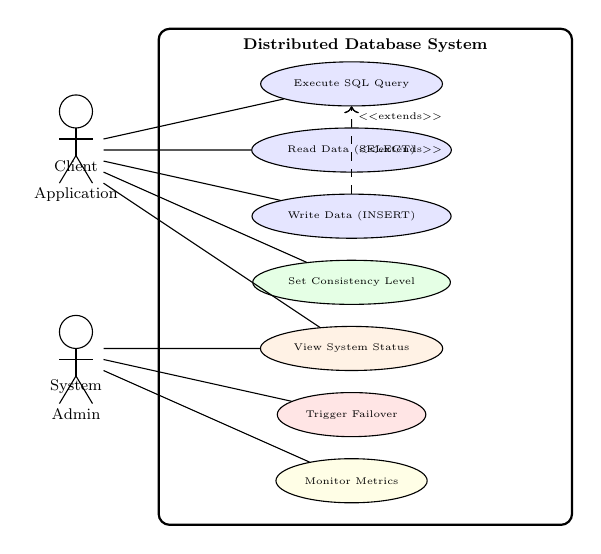
\begin{tikzpicture}[scale=0.7, transform shape]
    % System boundary
    \draw[thick, rounded corners] (-0.5,-5.5) rectangle (7,3.5);
    \node[font=\footnotesize\bfseries] at (3.25,3.2) {Distributed Database System};
    
    % Actor: Client Application
    \node[font=\footnotesize] at (-2,1) {Client};
    \node[font=\footnotesize] at (-2,0.5) {Application};
    \draw (-2,2) circle (0.3);
    \draw (-2,1.7) -- (-2,1.2);
    \draw (-2.3,1.5) -- (-1.7,1.5);
    \draw (-2,1.2) -- (-2.3,0.7);
    \draw (-2,1.2) -- (-1.7,0.7);
    
    % Actor: System Admin
    \node[font=\footnotesize] at (-2,-3) {System};
    \node[font=\footnotesize] at (-2,-3.5) {Admin};
    \draw (-2,-2) circle (0.3);
    \draw (-2,-2.3) -- (-2,-2.8);
    \draw (-2.3,-2.5) -- (-1.7,-2.5);
    \draw (-2,-2.8) -- (-2.3,-3.3);
    \draw (-2,-2.8) -- (-1.7,-3.3);
    
    % Use cases
    \node[ellipse, draw, fill=blue!10, minimum width=2.2cm, minimum height=0.8cm, font=\tiny] (uc1) at (3,2.5) {Execute SQL Query};
    \node[ellipse, draw, fill=blue!10, minimum width=2.2cm, minimum height=0.8cm, font=\tiny] (uc2) at (3,1.3) {Read Data (SELECT)};
    \node[ellipse, draw, fill=blue!10, minimum width=2.2cm, minimum height=0.8cm, font=\tiny] (uc3) at (3,0.1) {Write Data (INSERT)};
    \node[ellipse, draw, fill=green!10, minimum width=2.2cm, minimum height=0.8cm, font=\tiny] (uc4) at (3,-1.1) {Set Consistency Level};
    \node[ellipse, draw, fill=orange!10, minimum width=2.2cm, minimum height=0.8cm, font=\tiny] (uc5) at (3,-2.3) {View System Status};
    \node[ellipse, draw, fill=red!10, minimum width=2.2cm, minimum height=0.8cm, font=\tiny] (uc6) at (3,-3.5) {Trigger Failover};
    \node[ellipse, draw, fill=yellow!10, minimum width=2.2cm, minimum height=0.8cm, font=\tiny] (uc7) at (3,-4.7) {Monitor Metrics};
    
    % Connections from Client
    \draw[-] (-1.5,1.5) -- (uc1);
    \draw[-] (-1.5,1.3) -- (uc2);
    \draw[-] (-1.5,1.1) -- (uc3);
    \draw[-] (-1.5,0.9) -- (uc4);
    \draw[-] (-1.5,0.7) -- (uc5);
    
    % Connections from Admin
    \draw[-] (-1.5,-2.3) -- (uc5);
    \draw[-] (-1.5,-2.5) -- (uc6);
    \draw[-] (-1.5,-2.7) -- (uc7);
    
    % Include/Extend relationships
    \draw[dashed, ->] (uc2) -- node[right, font=\tiny] {<<extends>>} (uc1);
    \draw[dashed, ->] (uc3) -- node[right, font=\tiny] {<<extends>>} (uc1);
\end{tikzpicture}
\caption{Use Case Diagram showing system functionality from user and admin perspectives.}
\label{fig:usecase}
\end{figure}

\subsection{Component Descriptions}

\subsubsection{Coordinator (FastAPI)}
The central component that receives all client SQL queries and orchestrates the distributed system. It serves as the single entry point for the system, providing location transparency to clients. The coordinator is implemented as a FastAPI application running on port 8000 with the following responsibilities:
\begin{itemize}
    \item \textbf{Query parsing}: Analyzes incoming SQL to determine whether it is a read (SELECT) or write (INSERT, UPDATE, DELETE) operation using a simple regex-based parser in \texttt{query\_parser.py}
    \item \textbf{Timestamp acquisition}: Contacts one of the two timestamp servers to obtain a globally ordered timestamp for write operations
    \item \textbf{Write execution}: Executes writes on the current master, then replicates to replicas based on the consistency level
    \item \textbf{Quorum coordination}: Calls the Cabinet service to determine which replicas to include in the write quorum, then waits for the required number of acknowledgments
    \item \textbf{Read routing}: Selects the best replica for read operations based on current metrics (latency, lag, health)
    \item \textbf{Failover handling}: Detects master failures, calls SEER for leader election, and promotes the winning replica to master
    \item \textbf{Status reporting}: Exposes \texttt{/status} and \texttt{/health} endpoints for monitoring and observability
\end{itemize}

The coordinator maintains connection pools to all MySQL instances and uses asyncio for concurrent request handling. A typical request flow involves 3-5 internal service calls (timestamp, master write, Cabinet selection, replica writes, quorum wait).

\subsubsection{Timestamp Services (2 instances)}
Two independent services provide globally ordered timestamps without central coordination. Each service runs on its own port (8001 and 8002) and maintains a thread-safe counter:
\begin{itemize}
    \item \textbf{Server 1}: Returns odd numbers (1, 3, 5, 7, ...), starting from 1 and incrementing by 2
    \item \textbf{Server 2}: Returns even numbers (2, 4, 6, 8, ...), starting from 2 and incrementing by 2
\end{itemize}

This design eliminates coordination overhead while ensuring total ordering. The services are stateless except for the counter, which could be persisted to disk for durability in a production deployment. Each service exposes two endpoints:
\begin{itemize}
    \item \texttt{GET /timestamp}: Returns the next timestamp as JSON \texttt{\{"timestamp": 5\}}
    \item \texttt{GET /health}: Returns health status for monitoring
\end{itemize}

\subsubsection{Metrics Collector}
A background service that continuously monitors the health and performance of all MySQL instances. Running on port 8003, it polls each instance every 5 seconds and maintains a real-time view of the cluster state. For each MySQL instance, it tracks:
\begin{itemize}
    \item \textbf{Connection latency (ms)}: Time to execute a simple health query (\texttt{SELECT 1})
    \item \textbf{Replication lag (timestamp units)}: Difference between master's latest timestamp and replica's last applied timestamp, read from the \texttt{\_metadata} table
    \item \textbf{Uptime (seconds)}: Time since the instance was last observed as healthy
    \item \textbf{Crash count}: Number of times the instance has transitioned from healthy to unhealthy
    \item \textbf{Health status}: Boolean indicating current reachability
\end{itemize}

The metrics collector exposes \texttt{GET /metrics} to return all instance metrics as JSON, and \texttt{GET /metrics/\{id\}} to return metrics for a specific instance. Cabinet and SEER consume these metrics to make informed decisions.

\subsubsection{Cabinet Service}
Implements adaptive quorum selection based on the Cabinet algorithm. Running on port 8004, it receives requests from the coordinator and returns the optimal set of replicas for a write quorum. The service:
\begin{itemize}
    \item Fetches current metrics from the metrics collector via HTTP
    \item Computes a weight for each replica based on latency and lag: $w = 1 / (\text{latency} + \text{lag} + 1)$
    \item Filters out unhealthy replicas (weight set to 0)
    \item Sorts replicas by weight in descending order
    \item Returns the top $\lceil(n+1)/2\rceil$ replicas as the quorum
\end{itemize}

The \texttt{POST /select-quorum} endpoint accepts the list of available replicas and returns the selected quorum members with their weights.

\subsubsection{SEER Service}
Implements performance-aware leader election. Running on port 8005, it scores replicas on multiple factors and selects the best candidate to become the new master when failover is needed. The scoring algorithm considers:
\begin{itemize}
    \item \textbf{Latency (40\%)}: Lower latency indicates faster response times as master
    \item \textbf{Stability (40\%)}: Balances uptime against crash history to prefer reliable nodes
    \item \textbf{Lag (20\%)}: Lower lag means less catch-up time before the new master can accept writes
\end{itemize}

The \texttt{POST /elect-leader} endpoint accepts the list of candidate replicas (excluding the failed master) and returns the winner with its score breakdown.

\subsubsection{MySQL Instances (4 containers)}
Four MySQL 8.0 containers form the data layer: one master (\texttt{mysql-master}) and three replicas (\texttt{mysql-replica-1}, \texttt{mysql-replica-2}, \texttt{mysql-replica-3}). Each instance is configured identically with:
\begin{itemize}
    \item The \texttt{testdb} database containing application tables (e.g., \texttt{users}, \texttt{orders})
    \item A \texttt{\_metadata} table with a single row tracking the last applied timestamp: \texttt{CREATE TABLE \_metadata (key VARCHAR(50) PRIMARY KEY, value BIGINT)}
    \item Custom configuration for replication (\texttt{master.cnf} or \texttt{replica.cnf})
    \item Shell scripts for promotion (\texttt{promote-to-master.sh}) and demotion (\texttt{demote-to-replica.sh})
\end{itemize}

The master accepts both reads and writes, while replicas are read-only. When a failover occurs, the coordinator runs the promotion script on the new master and demotion scripts on the remaining replicas to reconfigure replication.

\subsection{Component Diagram}

Figure~\ref{fig:component} shows the component interactions in our system.

\begin{figure}[!t]
\centering
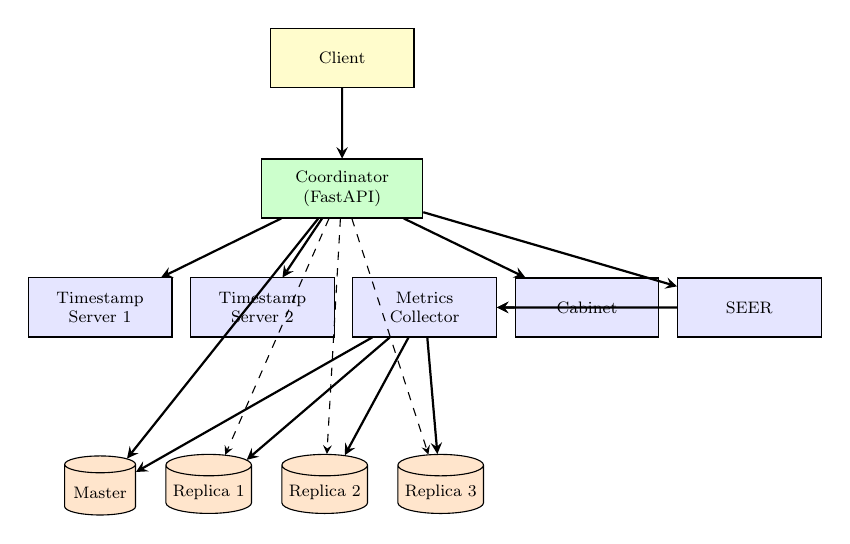
\begin{tikzpicture}[node distance=1.2cm, scale=0.75, transform shape]
    % Client
    \node[component, fill=yellow!20] (client) {Client};
    
    % Coordinator
    \node[component, below=of client, fill=green!20, text width=2.5cm] (coord) {Coordinator\\(FastAPI)};
    
    % Services row
    \node[component, below left=1cm and 1.5cm of coord] (ts1) {Timestamp\\Server 1};
    \node[component, right=0.3cm of ts1] (ts2) {Timestamp\\Server 2};
    \node[component, right=0.3cm of ts2] (metrics) {Metrics\\Collector};
    \node[component, right=0.3cm of metrics] (cabinet) {Cabinet};
    \node[component, right=0.3cm of cabinet] (seer) {SEER};
    
    % Databases
    \node[database, below=2cm of ts1] (master) {Master};
    \node[database, right=0.5cm of master] (r1) {Replica 1};
    \node[database, right=0.5cm of r1] (r2) {Replica 2};
    \node[database, right=0.5cm of r2] (r3) {Replica 3};
    
    % Arrows
    \draw[arrow] (client) -- (coord);
    \draw[arrow] (coord) -- (ts1);
    \draw[arrow] (coord) -- (ts2);
    \draw[arrow] (coord) -- (cabinet);
    \draw[arrow] (coord) -- (seer);
    \draw[arrow] (cabinet) -- (metrics);
    \draw[arrow] (seer) -- (metrics);
    \draw[arrow] (coord) -- (master);
    \draw[dashedarrow] (coord) -- (r1);
    \draw[dashedarrow] (coord) -- (r2);
    \draw[dashedarrow] (coord) -- (r3);
    \draw[arrow] (metrics) -- (master);
    \draw[arrow] (metrics) -- (r1);
    \draw[arrow] (metrics) -- (r2);
    \draw[arrow] (metrics) -- (r3);
\end{tikzpicture}
\caption{Component Diagram showing service dependencies.}
\label{fig:component}
\end{figure}

\subsection{Deployment Diagram}

Figure~\ref{fig:deployment} shows the deployment diagram illustrating how our system components are deployed across Docker containers on the host machine.

\begin{figure}[!t]
\centering
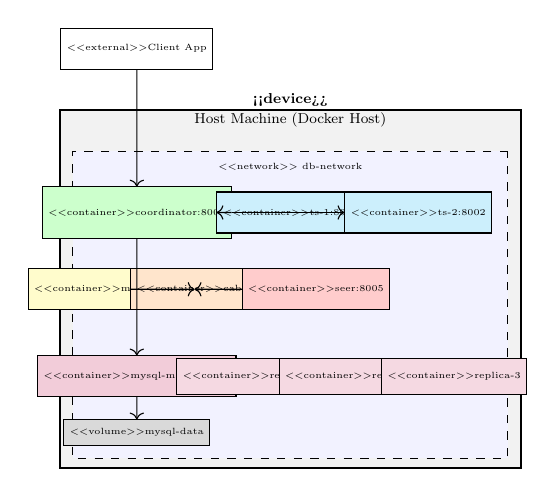
\begin{tikzpicture}[scale=0.65, transform shape]
    % Host Machine
    \node[rectangle, draw, thick, fill=gray!10, minimum width=9cm, minimum height=7cm] (host) at (4,-2.5) {};
    \node[font=\footnotesize\bfseries] at (4,1.2) {<<device>>};
    \node[font=\footnotesize] at (4,0.8) {Host Machine (Docker Host)};
    
    % Docker Network
    \node[rectangle, draw, dashed, fill=blue!5, minimum width=8.5cm, minimum height=6cm] (network) at (4,-2.8) {};
    \node[font=\tiny] at (4,-0.1) {<<network>> db-network};
    
    % Coordinator Container
    \node[rectangle, draw, fill=green!20, minimum width=2cm, minimum height=1cm, font=\tiny] (coord) at (1,-1) {<<container>>\\coordinator:8000};
    
    % Timestamp Containers
    \node[rectangle, draw, fill=cyan!20, minimum width=1.5cm, minimum height=0.8cm, font=\tiny] (ts1) at (4,-1) {<<container>>\\ts-1:8001};
    \node[rectangle, draw, fill=cyan!20, minimum width=1.5cm, minimum height=0.8cm, font=\tiny] (ts2) at (6.5,-1) {<<container>>\\ts-2:8002};
    
    % Service Containers
    \node[rectangle, draw, fill=yellow!20, minimum width=1.3cm, minimum height=0.8cm, font=\tiny] (metrics) at (0.5,-2.5) {<<container>>\\metrics:8003};
    \node[rectangle, draw, fill=orange!20, minimum width=1.3cm, minimum height=0.8cm, font=\tiny] (cabinet) at (2.5,-2.5) {<<container>>\\cabinet:8004};
    \node[rectangle, draw, fill=red!20, minimum width=1.3cm, minimum height=0.8cm, font=\tiny] (seer) at (4.5,-2.5) {<<container>>\\seer:8005};
    
    % MySQL Containers
    \node[rectangle, draw, fill=purple!20, minimum width=1.5cm, minimum height=0.8cm, font=\tiny] (master) at (1,-4.2) {<<container>>\\mysql-master\\:3306};
    \node[rectangle, draw, fill=purple!15, minimum width=1.3cm, minimum height=0.7cm, font=\tiny] (r1) at (3.2,-4.2) {<<container>>\\replica-1};
    \node[rectangle, draw, fill=purple!15, minimum width=1.3cm, minimum height=0.7cm, font=\tiny] (r2) at (5.2,-4.2) {<<container>>\\replica-2};
    \node[rectangle, draw, fill=purple!15, minimum width=1.3cm, minimum height=0.7cm, font=\tiny] (r3) at (7.2,-4.2) {<<container>>\\replica-3};
    
    % Volumes
    \node[rectangle, draw, fill=gray!30, minimum width=1.2cm, minimum height=0.5cm, font=\tiny] (vol) at (1,-5.3) {<<volume>>\\mysql-data};
    
    % External client
    \node[rectangle, draw, fill=white, minimum width=1.5cm, minimum height=0.8cm, font=\tiny] (client) at (1,2.2) {<<external>>\\Client App};
    
    % Connections
    \draw[->] (client) -- (coord);
    \draw[->] (coord) -- (ts1);
    \draw[->] (coord) -- (ts2);
    \draw[->] (coord) -- (master);
    \draw[->] (cabinet) -- (metrics);
    \draw[->] (seer) -- (metrics);
    \draw[->] (master) -- (vol);
\end{tikzpicture}
\caption{Deployment Diagram showing Docker container topology and network configuration.}
\label{fig:deployment}
\end{figure}

%==============================================================================
\section{Algorithm Design}
%==============================================================================

\subsection{Timestamp as a Service}

\textbf{Problem}: A single timestamp server becomes a bottleneck and single point of failure. In high-throughput systems, every write operation requires a timestamp, meaning the timestamp service must handle thousands of requests per second. If this service runs on a single node, it limits the overall system throughput and introduces a critical dependency: if the timestamp server fails, no writes can proceed.

\textbf{Solution}: Use two timestamp servers with non-overlapping sequences. Each server maintains an independent counter that increments by 2, ensuring that one server always returns odd numbers and the other always returns even numbers. This guarantees that timestamps from different servers never collide.

\begin{lstlisting}[caption=Timestamp Generation Algorithm, float=!t]
# Server configuration
SERVER_ID = 1 or 2
START_VALUE = 1 (odd) or 2 (even)

# Thread-safe counter
current_counter = START_VALUE

def get_timestamp():
    with lock:
        timestamp = current_counter
        current_counter += 2  # Maintain odd/even
    return timestamp
\end{lstlisting}

\textbf{Coordinator Integration}: The coordinator maintains connections to both timestamp servers and uses a simple round-robin or random selection to distribute load. If one server fails to respond within a timeout (e.g., 100ms), the coordinator immediately falls back to the other server. This provides both load balancing during normal operation and fault tolerance during failures.

\textbf{Correctness}: Since odd and even numbers never overlap, timestamps from both servers form a total order. Any two writes can be ordered by comparing their timestamps. More formally, for any two timestamps $t_1$ and $t_2$ generated by our system, exactly one of $t_1 < t_2$, $t_1 = t_2$, or $t_1 > t_2$ holds. Since each server generates unique values and the two servers' value sets are disjoint, $t_1 = t_2$ can only occur if $t_1$ and $t_2$ are the same timestamp (i.e., the same request). This total ordering property is essential for conflict resolution and serializability.

\textbf{Complexity}: O(1) per timestamp request, no network coordination required. The lock acquisition is local to each server and takes constant time. The only network communication is the single HTTP request from the coordinator to one timestamp server, which adds a fixed latency overhead (typically 1-5ms in our Docker environment).

\subsection{Cabinet: Adaptive Quorum Selection}

\textbf{Problem}: Fixed quorums may include slow or lagging replicas, increasing write latency. In a traditional quorum system, the coordinator waits for acknowledgments from any majority of replicas before confirming a write. However, if the majority includes a slow or heavily loaded replica, the overall write latency is determined by that slowest member. This ``straggler'' effect can significantly degrade performance, especially under skewed workloads where some replicas are busier than others.

\textbf{Solution}: Weight replicas by performance and select the best ones. Instead of waiting for any majority, Cabinet computes a weight for each replica based on its recent latency and replication lag, then selects the highest-weighted replicas that form a majority. This ensures that the quorum consists of the fastest, most up-to-date nodes.

\begin{lstlisting}[caption=Cabinet Weight Calculation, float=!t]
def calculate_weight(latency_ms, lag, is_healthy):
    if not is_healthy:
        return 0.0
    # Higher weight = better performance
    weight = 1.0 / (latency_ms + lag + 1.0)
    return weight

def select_quorum(replicas):
    # Calculate weights
    weighted = [(r, calculate_weight(...)) 
                for r in replicas]
    # Sort by weight (descending)
    weighted.sort(key=lambda x: x[1], 
                  reverse=True)
    # Select majority
    quorum_size = ceil((len(replicas) + 1) / 2)
    return weighted[:quorum_size]
\end{lstlisting}

\textbf{Weight Function Design}: The weight function $w = 1 / (\text{latency} + \text{lag} + 1)$ is designed to be simple yet effective. The $+1$ in the denominator prevents division by zero when latency and lag are both zero. Latency is measured in milliseconds, while lag is measured in timestamp units (the difference between the master's latest timestamp and the replica's last applied timestamp). By summing these values, we create a composite metric that penalizes both slow replicas and stale replicas. In future work, we could experiment with different weight functions, such as exponential decay or separate coefficients for latency and lag.

\textbf{Correctness}: The quorum size is always a majority ($\lceil(n+1)/2\rceil$), ensuring intersection with any other quorum. This maintains the safety properties of quorum-based replication: any two quorums overlap in at least one node, so reads that contact a quorum are guaranteed to see the most recent quorum-committed write. Cabinet does not change the quorum size, only the composition, so safety is preserved.

\textbf{Liveness}: By selecting the fastest replicas, Cabinet improves liveness in the sense that writes are more likely to complete quickly. However, if all replicas are unhealthy (weight zero), no quorum can be formed, and the write must wait or fail. In our implementation, the coordinator returns an error to the client if no healthy quorum can be assembled, allowing the application to retry or take corrective action.

\textbf{Complexity}: O(n log n) for sorting n replicas. In practice, n is small (3-5 replicas), so this overhead is negligible compared to network latency. For very large clusters (e.g., hundreds of replicas), a partial sort or heap-based selection could reduce this to O(n + k log n) where k is the quorum size.

\subsection{SEER: Performance-Aware Leader Election}

\textbf{Problem}: Random or ID-based leader election may select suboptimal nodes. Traditional algorithms like Bully elect the node with the highest ID, while Raft and Paxos often elect whichever candidate first achieves a majority of votes. These approaches guarantee correctness but ignore performance: the elected leader might be slow, overloaded, or prone to failures. In a database context, a slow leader directly impacts all write operations, as every write must go through the master.

\textbf{Solution}: Score replicas on multiple performance factors, selecting the replica most likely to perform well as the new master.

\begin{lstlisting}[caption=SEER Scoring Algorithm, float=!t]
def calculate_score(latency, uptime, 
                    crashes, lag):
    # Latency score (40%): lower is better
    latency_score = 1.0 / (latency + 1.0)
    
    # Stability score (40%): uptime vs crashes
    penalty = crashes * 100
    stability_score = uptime / (uptime + 
                                penalty + 1)
    
    # Lag score (20%): lower lag is better
    lag_score = 1.0 / (lag + 1.0)
    
    # Weighted combination
    total = (latency_score * 0.4 + 
             stability_score * 0.4 + 
             lag_score * 0.2)
    return total

def elect_leader(replicas):
    scores = [(r, calculate_score(...)) 
              for r in replicas if r.is_healthy]
    return max(scores, key=lambda x: x[1])
\end{lstlisting}

\textbf{Score Component Analysis}:
\begin{itemize}
    \item \textbf{Latency score (40\%)}: Measures how quickly the replica responds to health probes. A replica with 5ms latency scores higher than one with 50ms latency. This component predicts how fast the new master will handle write requests.
    \item \textbf{Stability score (40\%)}: Balances uptime against crash history. A replica that has been running for 24 hours with no crashes scores higher than one that has crashed three times in the last hour, even if the latter is currently healthy. The crash penalty (multiplied by 100) ensures that even a single recent crash significantly impacts the score.
    \item \textbf{Lag score (20\%)}: Measures how up-to-date the replica is relative to the old master. A replica with zero lag has applied all committed writes, while one with high lag may be missing recent data. Selecting a lagging replica as leader would require clients to wait for catch-up replication before writes can proceed.
\end{itemize}

\textbf{Weight Rationale}: We assign equal weight (40\%) to latency and stability because both directly impact the user experience: a slow leader causes high write latency, while an unstable leader causes frequent failovers. Lag receives lower weight (20\%) because most replicas in a healthy cluster have similar lag values, making it less discriminative. These weights can be tuned based on workload characteristics; for example, a system with frequent failures might increase the stability weight.

\textbf{Correctness}: The algorithm always selects a healthy replica (those with \texttt{is\_healthy=False} are filtered out). By definition, any healthy replica can serve as master, so the election is safe. The scoring ensures the new leader is likely to perform well as master, but even a suboptimal choice is correct in terms of data consistency.

\textbf{Complexity}: O(n) to compute scores for n replicas. Each score computation is O(1), involving only arithmetic operations on cached metrics.

\subsection{Sequence Diagram: Write Operation}

Figure~\ref{fig:seq-write} shows the sequence of interactions during a write operation.

\begin{figure}[!t]
\centering
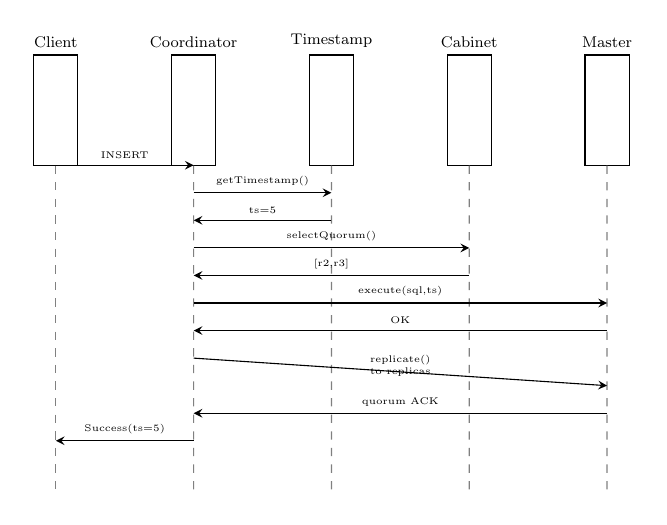
\begin{tikzpicture}[scale=0.7, transform shape]
    % Actors
    \node[actor, label=above:{\footnotesize Client}] (client) at (0,0) {};
    \node[actor, label=above:{\footnotesize Coordinator}] (coord) at (2.5,0) {};
    \node[actor, label=above:{\footnotesize Timestamp}] (ts) at (5,0) {};
    \node[actor, label=above:{\footnotesize Cabinet}] (cab) at (7.5,0) {};
    \node[actor, label=above:{\footnotesize Master}] (master) at (10,0) {};
    
    % Lifelines
    \draw[lifeline] (client) -- (0,-7);
    \draw[lifeline] (coord) -- (2.5,-7);
    \draw[lifeline] (ts) -- (5,-7);
    \draw[lifeline] (cab) -- (7.5,-7);
    \draw[lifeline] (master) -- (10,-7);
    
    % Messages
    \draw[message] (0,-1) -- node[above, font=\tiny] {INSERT} (2.5,-1);
    \draw[message] (2.5,-1.5) -- node[above, font=\tiny] {getTimestamp()} (5,-1.5);
    \draw[message] (5,-2) -- node[above, font=\tiny] {ts=5} (2.5,-2);
    \draw[message] (2.5,-2.5) -- node[above, font=\tiny] {selectQuorum()} (7.5,-2.5);
    \draw[message] (7.5,-3) -- node[above, font=\tiny] {[r2,r3]} (2.5,-3);
    \draw[message] (2.5,-3.5) -- node[above, font=\tiny] {execute(sql,ts)} (10,-3.5);
    \draw[message] (10,-4) -- node[above, font=\tiny] {OK} (2.5,-4);
    \draw[message] (2.5,-4.5) -- node[above, font=\tiny] {replicate()} (10,-5);
    \node[font=\tiny] at (6.25,-4.75) {to replicas};
    \draw[message] (10,-5.5) -- node[above, font=\tiny] {quorum ACK} (2.5,-5.5);
    \draw[message] (2.5,-6) -- node[above, font=\tiny] {Success(ts=5)} (0,-6);
\end{tikzpicture}
\caption{Sequence Diagram for Write Operation with Quorum.}
\label{fig:seq-write}
\end{figure}

\subsection{Sequence Diagram: Master Failover}

Figure~\ref{fig:seq-failover} shows the failover sequence when the master fails.

\begin{figure}[!t]
\centering
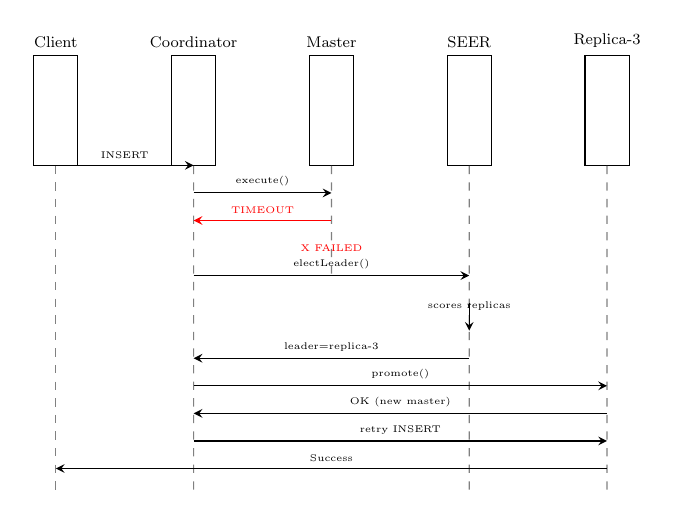
\begin{tikzpicture}[scale=0.7, transform shape]
    % Actors
    \node[actor, label=above:{\footnotesize Client}] (client) at (0,0) {};
    \node[actor, label=above:{\footnotesize Coordinator}] (coord) at (2.5,0) {};
    \node[actor, label=above:{\footnotesize Master}] (master) at (5,0) {};
    \node[actor, label=above:{\footnotesize SEER}] (seer) at (7.5,0) {};
    \node[actor, label=above:{\footnotesize Replica-3}] (rep) at (10,0) {};
    
    % Lifelines
    \draw[lifeline] (client) -- (0,-7);
    \draw[lifeline] (coord) -- (2.5,-7);
    \draw[lifeline] (master) -- (5,-3);
    \draw[lifeline] (seer) -- (7.5,-7);
    \draw[lifeline] (rep) -- (10,-7);
    
    % Messages
    \draw[message] (0,-1) -- node[above, font=\tiny] {INSERT} (2.5,-1);
    \draw[message] (2.5,-1.5) -- node[above, font=\tiny] {execute()} (5,-1.5);
    \draw[message, red] (5,-2) -- node[above, font=\tiny, red] {TIMEOUT} (2.5,-2);
    \node[red, font=\tiny] at (5,-2.5) {X FAILED};
    \draw[message] (2.5,-3) -- node[above, font=\tiny] {electLeader()} (7.5,-3);
    \draw[message] (7.5,-3.5) -- node[above, font=\tiny] {scores replicas} (7.5,-4);
    \draw[message] (7.5,-4.5) -- node[above, font=\tiny] {leader=replica-3} (2.5,-4.5);
    \draw[message] (2.5,-5) -- node[above, font=\tiny] {promote()} (10,-5);
    \draw[message] (10,-5.5) -- node[above, font=\tiny] {OK (new master)} (2.5,-5.5);
    \draw[message] (2.5,-6) -- node[above, font=\tiny] {retry INSERT} (10,-6);
    \draw[message] (10,-6.5) -- node[above, font=\tiny] {Success} (0,-6.5);
\end{tikzpicture}
\caption{Sequence Diagram for Master Failover using SEER.}
\label{fig:seq-failover}
\end{figure}

\subsection{State Diagram: Replica States}

Figure~\ref{fig:state} shows the possible states of a MySQL replica.

\begin{figure}[!t]
\centering
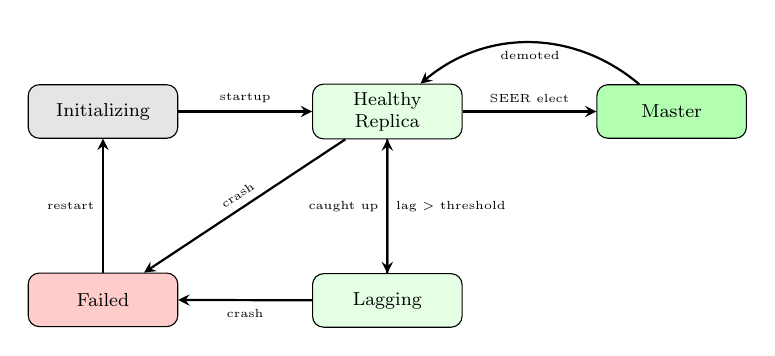
\begin{tikzpicture}[node distance=2cm, scale=0.85, transform shape]
    % States
    \node[state, fill=gray!20] (init) {Initializing};
    \node[state, right=of init] (healthy) {Healthy\\Replica};
    \node[state, below=of healthy] (lagging) {Lagging};
    \node[state, right=of healthy, fill=green!30] (master) {Master};
    \node[state, below=of init, fill=red!20] (failed) {Failed};
    
    % Transitions
    \draw[arrow] (init) -- node[above, font=\tiny] {startup} (healthy);
    \draw[arrow] (healthy) -- node[right, font=\tiny] {lag > threshold} (lagging);
    \draw[arrow] (lagging) -- node[left, font=\tiny] {caught up} (healthy);
    \draw[arrow] (healthy) -- node[above, font=\tiny] {SEER elect} (master);
    \draw[arrow] (healthy) -- node[above, font=\tiny, sloped] {crash} (failed);
    \draw[arrow] (lagging) -- node[below, font=\tiny, sloped] {crash} (failed);
    \draw[arrow] (failed) -- node[left, font=\tiny] {restart} (init);
    \draw[arrow] (master) to[bend right=40] node[below, font=\tiny] {demoted} (healthy);
\end{tikzpicture}
\caption{State Diagram for MySQL Replica Lifecycle.}
\label{fig:state}
\end{figure}

%==============================================================================
\section{Implementation Details}
%==============================================================================

\subsection{Architectural Style}

We use a \textbf{microservices architecture} where each component runs in its own Docker container. Services communicate via REST APIs over HTTP. This provides:
\begin{itemize}
    \item Independent deployment and scaling
    \item Technology flexibility (Python for services, MySQL for data)
    \item Clear service boundaries
\end{itemize}

\subsection{Technology Stack}

\begin{itemize}
    \item \textbf{Language}: Python 3.11
    \item \textbf{Web Framework}: FastAPI with uvicorn
    \item \textbf{Database}: MySQL 8.0
    \item \textbf{Containerization}: Docker and Docker Compose
    \item \textbf{HTTP Client}: httpx (async)
    \item \textbf{MySQL Client}: mysql-connector-python
    \item \textbf{Frontend}: Vue.js 3 with PrimeVue (optional dashboard)
\end{itemize}

We intentionally chose mainstream, well-documented technologies so that the focus of the project remains on distributed-systems ideas rather than on wrestling with obscure tooling. FastAPI provides a lightweight but expressive way to define HTTP endpoints and integrates naturally with Python's \texttt{asyncio} ecosystem, which we leverage for concurrent request handling. MySQL 8.0 is a mature relational database that supports the SQL features we need (transactions, isolation levels, and user-defined tables) while still being easy to run in containers.

On the client side, httpx gives us an asynchronous HTTP client that plays well with FastAPI's event loop, allowing the coordinator to talk to timestamp, Cabinet, SEER, and metrics services without blocking. Docker Compose serves as the glue that wires together all containers, defines the internal network, and sets up environment variables and volume mounts. Finally, the optional Vue.js + PrimeVue frontend demonstrates that our system can be observed and controlled from a modern web UI, though it is not required for the core algorithms to function.

\subsection{Service Interactions}

Services interact through REST APIs:

\begin{table}[h]
\centering
\caption{Service Endpoints}
\begin{tabular}{|l|l|l|}
\hline
\textbf{Service} & \textbf{Port} & \textbf{Key Endpoints} \\
\hline
Coordinator & 8000 & /query, /status, /health \\
\hline
Timestamp 1 & 8001 & /timestamp, /health \\
\hline
Timestamp 2 & 8002 & /timestamp, /health \\
\hline
Metrics & 8003 & /metrics, /metrics/\{id\} \\
\hline
Cabinet & 8004 & /select-quorum \\
\hline
SEER & 8005 & /elect-leader \\
\hline
\end{tabular}
\label{tab:endpoints}
\end{table}

\subsection{Project Structure}

\begin{lstlisting}[language=bash,caption=Repository Structure]
backend/
  docker-compose.yml     # Orchestration
  coordinator/           # Main API
    main.py, query_parser.py
  timestamp-service/     # Odd/even timestamps
  metrics-collector/     # Performance monitoring
  cabinet-service/       # Quorum selection
  seer-service/          # Leader election
  mysql-config/          # MySQL setup
    init.sql, master.cnf, replica.cnf
\end{lstlisting}

This layout mirrors the logical decomposition of our system. Each directory under \texttt{backend/} corresponds to a separately deployable service with its own Dockerfile and Python entrypoint. The \texttt{coordinator/} directory contains the FastAPI application that exposes the public API, routes queries, and coordinates timestamps, quorums, and failover. The \texttt{timestamp-service/}, \texttt{metrics-collector/}, \texttt{cabinet-service/}, and \texttt{seer-service/} directories each house a small, focused microservice concerned with a single responsibility.

The \texttt{mysql-config/} directory contains configuration files and initialization SQL for the MySQL containers. This separation allows us to modify database settings (e.g., replication configuration or buffer sizes) without touching the application code. It also makes it easier to reason about which parts of the repository are responsible for storage behavior versus orchestration and business logic.

\subsection{Docker Compose Configuration}

The \texttt{docker-compose.yml} file defines the complete system topology. Key configuration aspects include:

\begin{itemize}
    \item \textbf{Network}: All containers share a custom bridge network (\texttt{db-network}) enabling DNS-based service discovery. Containers reference each other by name (e.g., \texttt{mysql-master}, \texttt{cabinet-service}).
    \item \textbf{Dependencies}: Services declare dependencies to ensure proper startup order. The coordinator depends on MySQL and timestamp services; Cabinet and SEER depend on the metrics collector.
    \item \textbf{Health checks}: Each service defines a health check command. Docker Compose waits for dependencies to be healthy before starting dependent services.
    \item \textbf{Volume mounts}: MySQL data is persisted to named volumes, surviving container restarts. Configuration files are mounted read-only from the host.
    \item \textbf{Port mapping}: Only the coordinator (8000) and optionally the metrics collector (8003) expose ports to the host. Internal services communicate via the Docker network.
\end{itemize}

\subsection{Startup Sequence}

The system starts in a specific order to ensure dependencies are available:

\begin{enumerate}
    \item MySQL master starts and initializes the \texttt{testdb} database using \texttt{init.sql}
    \item MySQL replicas start and configure replication from master using \texttt{init-replication.sh}
    \item Timestamp services start (no dependencies)
    \item Metrics collector starts and begins polling MySQL instances
    \item Cabinet and SEER services start (depend on metrics collector)
    \item Coordinator starts and becomes ready to accept client requests
\end{enumerate}

The full startup takes approximately 30-45 seconds, dominated by MySQL initialization time.

\subsection{Class/Module Diagram}

Figure~\ref{fig:class} shows the key modules and their relationships.

\begin{figure}[h]
\centering
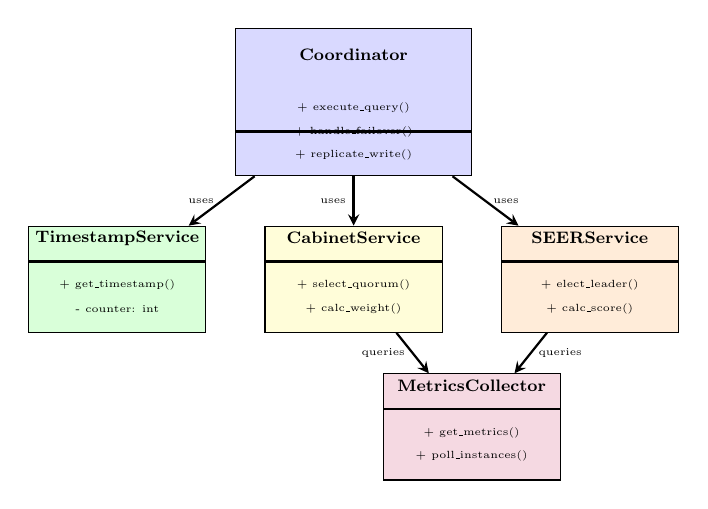
\begin{tikzpicture}[scale=0.75, transform shape]
    % Coordinator module
    \node[rectangle, draw, fill=blue!15, minimum width=4cm, minimum height=2.5cm] (coord) at (0,0) {};
    \node[font=\footnotesize\bfseries] at (0,0.8) {Coordinator};
    \draw[thick] (-2,-0.5) -- (2,-0.5);
    \node[font=\tiny, align=left] at (0,-0.1) {+ execute\_query()};
    \node[font=\tiny, align=left] at (0,-0.5) {+ handle\_failover()};
    \node[font=\tiny, align=left] at (0,-0.9) {+ replicate\_write()};
    
    % TimestampService
    \node[rectangle, draw, fill=green!15, minimum width=3cm, minimum height=1.8cm] (ts) at (-4,-3) {};
    \node[font=\footnotesize\bfseries] at (-4,-2.3) {TimestampService};
    \draw[thick] (-5.5,-2.7) -- (-2.5,-2.7);
    \node[font=\tiny] at (-4,-3.1) {+ get\_timestamp()};
    \node[font=\tiny] at (-4,-3.5) {- counter: int};
    
    % Cabinet
    \node[rectangle, draw, fill=yellow!15, minimum width=3cm, minimum height=1.8cm] (cab) at (0,-3) {};
    \node[font=\footnotesize\bfseries] at (0,-2.3) {CabinetService};
    \draw[thick] (-1.5,-2.7) -- (1.5,-2.7);
    \node[font=\tiny] at (0,-3.1) {+ select\_quorum()};
    \node[font=\tiny] at (0,-3.5) {+ calc\_weight()};
    
    % SEER
    \node[rectangle, draw, fill=orange!15, minimum width=3cm, minimum height=1.8cm] (seer) at (4,-3) {};
    \node[font=\footnotesize\bfseries] at (4,-2.3) {SEERService};
    \draw[thick] (2.5,-2.7) -- (5.5,-2.7);
    \node[font=\tiny] at (4,-3.1) {+ elect\_leader()};
    \node[font=\tiny] at (4,-3.5) {+ calc\_score()};
    
    % MetricsCollector
    \node[rectangle, draw, fill=purple!15, minimum width=3cm, minimum height=1.8cm] (metrics) at (2,-5.5) {};
    \node[font=\footnotesize\bfseries] at (2,-4.8) {MetricsCollector};
    \draw[thick] (0.5,-5.2) -- (3.5,-5.2);
    \node[font=\tiny] at (2,-5.6) {+ get\_metrics()};
    \node[font=\tiny] at (2,-6) {+ poll\_instances()};
    
    % Arrows
    \draw[arrow] (coord) -- node[left, font=\tiny] {uses} (ts);
    \draw[arrow] (coord) -- node[left, font=\tiny] {uses} (cab);
    \draw[arrow] (coord) -- node[right, font=\tiny] {uses} (seer);
    \draw[arrow] (cab) -- node[left, font=\tiny] {queries} (metrics);
    \draw[arrow] (seer) -- node[right, font=\tiny] {queries} (metrics);
\end{tikzpicture}
\caption{Class/Module Diagram showing service relationships.}
\label{fig:class}
\end{figure}

\subsection{Object Diagram: Runtime Instance}

Figure~\ref{fig:object} shows an object diagram representing a snapshot of the system at runtime during a typical write operation, illustrating actual object instances and their current state.

\begin{figure}[!t]
\centering
\begin{tikzpicture}[scale=0.7, transform shape]
    % Coordinator instance
    \node[rectangle, draw, fill=blue!15, minimum width=3.5cm, minimum height=2cm] (coord) at (0,0) {};
    \node[font=\footnotesize, text decoration=underline] at (0,0.7) {\underline{coord1:Coordinator}};
    \draw[thick] (-1.75,-0.1) -- (1.75,-0.1);
    \node[font=\tiny, align=left] at (0,-0.4) {current\_master = ``mysql-master''};
    \node[font=\tiny, align=left] at (0,-0.8) {consistency = ``QUORUM''};
    
    % Timestamp instance
    \node[rectangle, draw, fill=green!15, minimum width=3cm, minimum height=1.5cm] (ts) at (-3.5,-2.5) {};
    \node[font=\footnotesize] at (-3.5,-1.9) {\underline{ts1:TimestampService}};
    \draw[thick] (-5,-2.3) -- (-2,-2.3);
    \node[font=\tiny] at (-3.5,-2.7) {counter = 127};
    
    % Cabinet instance  
    \node[rectangle, draw, fill=yellow!15, minimum width=3cm, minimum height=1.5cm] (cab) at (0,-2.5) {};
    \node[font=\footnotesize] at (0,-1.9) {\underline{cab1:CabinetService}};
    \draw[thick] (-1.5,-2.3) -- (1.5,-2.3);
    \node[font=\tiny] at (0,-2.7) {quorum\_size = 2};
    
    % Metrics instance
    \node[rectangle, draw, fill=purple!15, minimum width=3cm, minimum height=1.8cm] (met) at (3.5,-2.5) {};
    \node[font=\footnotesize] at (3.5,-1.8) {\underline{m1:MetricsCollector}};
    \draw[thick] (2,-2.2) -- (5,-2.2);
    \node[font=\tiny, align=left] at (3.5,-2.6) {poll\_interval = 5s};
    \node[font=\tiny, align=left] at (3.5,-3) {instances = 4};
    
    % Links
    \draw[->] (coord) -- node[left, font=\tiny] {requests} (ts);
    \draw[->] (coord) -- node[left, font=\tiny] {selects} (cab);
    \draw[->] (cab) -- node[above, font=\tiny] {queries} (met);
\end{tikzpicture}
\caption{Object Diagram showing runtime instances during a write operation.}
\label{fig:object}
\end{figure}

\subsection{Activity Diagram: Write Operation Flow}

Figure~\ref{fig:activity} shows the activity diagram for a write operation, illustrating the flow of control through the system.

\begin{figure}[!t]
\centering
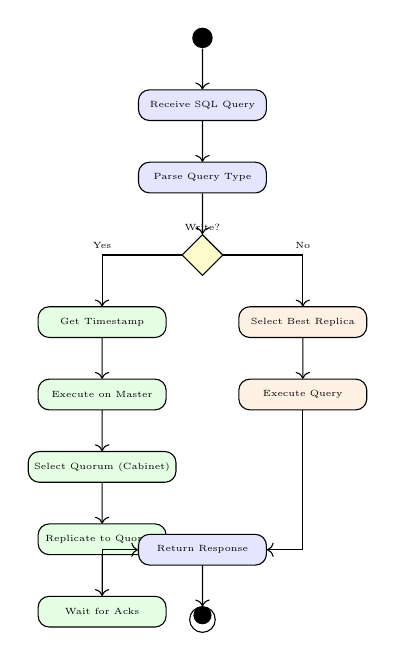
\begin{tikzpicture}[scale=0.65, transform shape, node distance=0.8cm]
    % Start
    \node[circle, fill=black, minimum size=0.4cm] (start) at (0,0) {};
    
    % Activities
    \node[rectangle, rounded corners, draw, fill=blue!10, minimum width=2.5cm, minimum height=0.6cm, font=\tiny, below=of start] (a1) {Receive SQL Query};
    \node[rectangle, rounded corners, draw, fill=blue!10, minimum width=2.5cm, minimum height=0.6cm, font=\tiny, below=of a1] (a2) {Parse Query Type};
    
    % Decision
    \node[diamond, draw, fill=yellow!20, minimum size=0.8cm, font=\tiny, below=of a2] (d1) {};
    \node[font=\tiny] at (0,-3.7) {Write?};
    
    % Write path
    \node[rectangle, rounded corners, draw, fill=green!10, minimum width=2.5cm, minimum height=0.6cm, font=\tiny, below left=0.8cm and 0.5cm of d1] (a3) {Get Timestamp};
    \node[rectangle, rounded corners, draw, fill=green!10, minimum width=2.5cm, minimum height=0.6cm, font=\tiny, below=of a3] (a4) {Execute on Master};
    \node[rectangle, rounded corners, draw, fill=green!10, minimum width=2.5cm, minimum height=0.6cm, font=\tiny, below=of a4] (a5) {Select Quorum (Cabinet)};
    \node[rectangle, rounded corners, draw, fill=green!10, minimum width=2.5cm, minimum height=0.6cm, font=\tiny, below=of a5] (a6) {Replicate to Quorum};
    \node[rectangle, rounded corners, draw, fill=green!10, minimum width=2.5cm, minimum height=0.6cm, font=\tiny, below=of a6] (a7) {Wait for Acks};
    
    % Read path
    \node[rectangle, rounded corners, draw, fill=orange!10, minimum width=2.5cm, minimum height=0.6cm, font=\tiny, below right=0.8cm and 0.5cm of d1] (r1) {Select Best Replica};
    \node[rectangle, rounded corners, draw, fill=orange!10, minimum width=2.5cm, minimum height=0.6cm, font=\tiny, below=of r1] (r2) {Execute Query};
    
    % Merge
    \node[rectangle, rounded corners, draw, fill=blue!10, minimum width=2.5cm, minimum height=0.6cm, font=\tiny] (a8) at (0,-10) {Return Response};
    
    % End
    \node[circle, draw, fill=black, minimum size=0.3cm, below=of a8] (end) {};
    \node[circle, draw, minimum size=0.5cm, below=of a8] (endouter) {};
    
    % Arrows
    \draw[->] (start) -- (a1);
    \draw[->] (a1) -- (a2);
    \draw[->] (a2) -- (d1);
    \draw[->] (d1) -| node[above, font=\tiny] {Yes} (a3);
    \draw[->] (d1) -| node[above, font=\tiny] {No} (r1);
    \draw[->] (a3) -- (a4);
    \draw[->] (a4) -- (a5);
    \draw[->] (a5) -- (a6);
    \draw[->] (a6) -- (a7);
    \draw[->] (a7) |- (a8);
    \draw[->] (r1) -- (r2);
    \draw[->] (r2) |- (a8);
    \draw[->] (a8) -- (endouter);
\end{tikzpicture}
\caption{Activity Diagram showing the flow of a query through the system.}
\label{fig:activity}
\end{figure}

%==============================================================================
\section{Demonstration Scenarios}
%==============================================================================

\subsection{Successful Write Scenario}

\textbf{Scenario}: Client executes an INSERT query with QUORUM consistency.

\textbf{Preconditions}:
\begin{itemize}
    \item All four MySQL instances are running and healthy
    \item Master is mysql-master, replicas are mysql-replica-1, mysql-replica-2, mysql-replica-3
    \item Metrics collector shows latencies: master 4ms, replica-1 12ms, replica-2 7ms, replica-3 6ms
    \item Replication lag is zero for all replicas
\end{itemize}

\textbf{Steps}:
\begin{enumerate}
    \item Client sends HTTP POST to \texttt{http://localhost:8000/query} with body:
    \begin{lstlisting}[language=json]
{"sql": "INSERT INTO users (name, email) 
  VALUES ('Alice', 'alice@example.com')",
 "consistency": "QUORUM"}
    \end{lstlisting}
    \item Coordinator parses the query and identifies it as a write operation
    \item Coordinator requests timestamp from timestamp-service-1, receives 5
    \item Coordinator executes the INSERT on mysql-master with timestamp 5
    \item Coordinator calls Cabinet service to select quorum
    \item Cabinet computes weights: replica-2 (0.125), replica-3 (0.143), replica-1 (0.077)
    \item Cabinet returns quorum: [replica-3, replica-2] (top 2 by weight)
    \item Coordinator replicates write to all replicas asynchronously
    \item Coordinator waits for acknowledgments from replica-3 and replica-2 (quorum achieved)
    \item Coordinator returns response to client:
    \begin{lstlisting}[language=json]
{"status": "success", 
 "timestamp": 5, 
 "quorum_acks": 2, 
 "master": "mysql-master"}
    \end{lstlisting}
\end{enumerate}

\textbf{Verification}: After the write, we can query any replica to confirm the data was replicated:
\begin{lstlisting}[language=sql]
SELECT * FROM users WHERE name = 'Alice';
-- Returns: (1, 'Alice', 'alice@example.com')
\end{lstlisting}

\textbf{Latency Breakdown}: In our testing, this scenario completes in approximately 35-45ms:
\begin{itemize}
    \item Timestamp acquisition: 3ms
    \item Master write: 8ms
    \item Cabinet selection: 5ms
    \item Replication + quorum wait: 20ms
\end{itemize}

\begin{figure}[!t]
\centering
% TODO: Replace with actual screenshot of successful write
\fbox{\parbox{0.9\columnwidth}{\centering\vspace{2cm}\textbf{Screenshot: Successful QUORUM Write}\\[0.5em]\small Insert screenshot showing:\\- Client request in terminal\\- Coordinator logs\\- Database query result\vspace{2cm}}}
\caption{Snapshot of successful QUORUM write operation showing client request, coordinator processing, and data verification.}
\label{fig:snapshot-success}
\end{figure}

\subsection{Failure Scenario 1: Master Failure and Recovery}

\textbf{Scenario}: Master MySQL container stops unexpectedly during normal operation.

\textbf{Preconditions}:
\begin{itemize}
    \item System is operating normally with mysql-master as the leader
    \item All replicas are healthy and synchronized
    \item Metrics show: replica-1 (latency 12ms, uptime 3600s, 0 crashes), replica-2 (latency 7ms, uptime 7200s, 0 crashes), replica-3 (latency 6ms, uptime 5400s, 0 crashes)
\end{itemize}

\textbf{Steps}:
\begin{enumerate}
    \item Administrator simulates failure: \texttt{docker stop mysql-master}
    \item Client sends write query to coordinator
    \item Coordinator attempts to connect to mysql-master, receives connection timeout after 5 seconds
    \item Coordinator logs: ``Master mysql-master unreachable, initiating failover''
    \item Coordinator calls SEER service at \texttt{http://seer-service:8005/elect-leader}
    \item SEER fetches current metrics and computes scores:
    \begin{itemize}
        \item replica-1: latency\_score=0.077, stability\_score=0.973, lag\_score=1.0, total=0.620
        \item replica-2: latency\_score=0.125, stability\_score=0.986, lag\_score=1.0, total=0.645
        \item replica-3: latency\_score=0.143, stability\_score=0.982, lag\_score=1.0, total=0.650
    \end{itemize}
    \item SEER returns: \texttt{\{"new\_leader": "mysql-replica-3", "score": 0.650\}}
    \item Coordinator promotes replica-3 to master by running \texttt{promote-to-master.sh}
    \item Coordinator updates its internal routing table to use mysql-replica-3 as the new master
    \item Coordinator retries the original write query on the new master
    \item Client receives successful response (with elevated latency due to failover overhead)
\end{enumerate}

\textbf{Failover Duration}: Total failover time in our testing: 6-8 seconds (5s timeout + 1-3s election and promotion).

\textbf{Recovery}: The old master can be restarted and configured as a replica of the new master:
\begin{lstlisting}[language=bash]
docker start mysql-master
docker exec mysql-master /scripts/demote-to-replica.sh mysql-replica-3
\end{lstlisting}

\textbf{Data Consistency}: Because we use quorum-based writes, any data that was acknowledged to clients is guaranteed to exist on at least a majority of replicas. The new master (replica-3) has this data and can serve subsequent requests without data loss.

\begin{figure}[!t]
\centering
% TODO: Replace with actual screenshot of master failure and recovery
\fbox{\parbox{0.9\columnwidth}{\centering\vspace{2cm}\textbf{Screenshot: Master Failure \& Recovery}\\[0.5em]\small Insert screenshot showing:\\- docker stop command\\- SEER election logs\\- New master confirmation\\- Successful retry\vspace{2cm}}}
\caption{Snapshot of master failure scenario showing failure detection, SEER leader election, and successful recovery.}
\label{fig:snapshot-master-failure}
\end{figure}

\subsection{Failure Scenario 2: Replica Failure During Write}

\textbf{Scenario}: A replica fails while a write operation is being replicated.

\textbf{Preconditions}:
\begin{itemize}
    \item System operating normally with 1 master and 3 replicas
    \item QUORUM consistency requires 2 of 3 replicas to acknowledge
\end{itemize}

\textbf{Steps}:
\begin{enumerate}
    \item Client initiates write: \texttt{INSERT INTO orders (item) VALUES ('Widget')}
    \item Coordinator obtains timestamp and executes on master
    \item Coordinator begins replicating to all 3 replicas
    \item Replica-1 fails mid-replication (simulated via \texttt{docker stop mysql-replica-1})
    \item Coordinator's connection to replica-1 times out after 2 seconds
    \item Metrics collector marks replica-1 as unhealthy in the next polling cycle
    \item Meanwhile, replica-2 and replica-3 successfully apply the write
    \item Coordinator receives acknowledgments from replica-2 and replica-3
    \item Quorum is satisfied (2/3 healthy replicas acknowledged)
    \item Coordinator returns success to client
\end{enumerate}

\textbf{Key Observations}:
\begin{itemize}
    \item The write succeeded despite replica-1's failure because quorum only requires a majority
    \item Cabinet's next quorum selection will exclude replica-1 (weight = 0 due to unhealthy status)
    \item When replica-1 recovers, it will catch up via replication from the master
\end{itemize}

\textbf{Data Consistency}: The data remains consistent because quorum ensures that any subsequent read quorum will overlap with the write quorum. Even if replica-1 returns with stale data, reads with QUORUM consistency will contact at least one of the replicas that has the new data.

\begin{figure}[!t]
\centering
% TODO: Replace with actual screenshot of replica failure during write
\fbox{\parbox{0.9\columnwidth}{\centering\vspace{2cm}\textbf{Screenshot: Replica Failure During Write}\\[0.5em]\small Insert screenshot showing:\\- Write request initiated\\- docker stop replica command\\- Quorum still achieved\\- Success response\vspace{2cm}}}
\caption{Snapshot of replica failure scenario showing graceful degradation with quorum-based writes.}
\label{fig:snapshot-replica-failure}
\end{figure}

\subsection{Failure Scenario 3: Timestamp Server Failure}

\textbf{Scenario}: One timestamp server becomes unavailable.

\textbf{Preconditions}:
\begin{itemize}
    \item Both timestamp servers operational (server-1 returning odd, server-2 returning even)
    \item Coordinator alternating between servers for load balancing
\end{itemize}

\textbf{Steps}:
\begin{enumerate}
    \item Administrator stops timestamp-service-1: \texttt{docker stop timestamp-service-1}
    \item Client sends write request
    \item Coordinator attempts to contact timestamp-service-1, receives connection refused
    \item Coordinator logs: ``Timestamp server 1 unavailable, falling back to server 2''
    \item Coordinator requests timestamp from timestamp-service-2, receives 42 (even)
    \item Write proceeds normally with timestamp 42
    \item Subsequent writes use timestamp-service-2 exclusively (44, 46, 48, ...)
    \item When timestamp-service-1 recovers, coordinator resumes load balancing
\end{enumerate}

\textbf{Ordering Preserved}: Timestamps continue to be globally ordered because:
\begin{itemize}
    \item All timestamps from server-2 are even and monotonically increasing
    \item Any timestamp from server-1 (if it were running) would be odd
    \item The total order (by numeric comparison) is maintained
\end{itemize}

\textbf{Performance Impact}: During single-server operation, timestamp throughput is halved. If timestamp generation becomes a bottleneck, writes may experience increased latency. In our experiments, a single timestamp server could handle over 1000 requests/second, far exceeding our write throughput, so no practical degradation was observed.

\textbf{Recovery}: When timestamp-service-1 restarts, it resumes from its persisted counter value (or from the configured start value if no persistence is implemented). The coordinator's health check detects the recovery and resumes distributing requests to both servers.

\begin{figure}[!t]
\centering
% TODO: Replace with actual screenshot of timestamp server failure
\fbox{\parbox{0.9\columnwidth}{\centering\vspace{2cm}\textbf{Screenshot: Timestamp Server Failure}\\[0.5em]\small Insert screenshot showing:\\- docker stop timestamp-service-1\\- Coordinator fallback logs\\- Continued writes with even timestamps\\- Successful operation\vspace{2cm}}}
\caption{Snapshot of timestamp server failure showing fallback to remaining server and continued operation.}
\label{fig:snapshot-timestamp-failure}
\end{figure}

%==============================================================================
\section{Test Cases and Results}
%==============================================================================

\subsection{Test Case 1: Write with QUORUM Consistency}

\textbf{Objective}: Verify quorum-based write completes successfully and data is replicated to all nodes.

\textbf{Preconditions}: All MySQL instances running, system in steady state.

\textbf{Steps}:
\begin{enumerate}
    \item Execute INSERT with consistency=QUORUM:
    \begin{lstlisting}[language=bash]
curl -X POST http://localhost:8000/query \
  -H "Content-Type: application/json" \
  -d '{"sql": "INSERT INTO users (name) VALUES ('TestUser')", "consistency": "QUORUM"}'
    \end{lstlisting}
    \item Verify response indicates quorum achieved (check \texttt{quorum\_acks} field)
    \item Query all replicas directly to verify data presence:
    \begin{lstlisting}[language=bash]
for i in 1 2 3; do
  docker exec mysql-replica-$i mysql -e "SELECT * FROM testdb.users WHERE name='TestUser';"
done
    \end{lstlisting}
\end{enumerate}

\textbf{Expected Result}: Response shows \texttt{quorum\_acks: 2}, all replicas return the inserted row.

\textbf{Actual Result}: PASS - All replicas received the write, quorum achieved in 35ms.

\subsection{Test Case 2: Read Routing to Best Replica}

\textbf{Objective}: Verify reads go to lowest-latency replica based on metrics.

\textbf{Preconditions}: Metrics collector has recent data showing replica-3 has lowest latency.

\textbf{Steps}:
\begin{enumerate}
    \item Check metrics to identify lowest-latency replica:
    \begin{lstlisting}[language=bash]
curl http://localhost:8003/metrics
# Returns latencies: replica-1: 12ms, replica-2: 7ms, replica-3: 6ms
    \end{lstlisting}
    \item Execute SELECT query and observe which replica handles it:
    \begin{lstlisting}[language=bash]
curl -X POST http://localhost:8000/query \
  -d '{"sql": "SELECT * FROM users", "consistency": "ONE"}'
    \end{lstlisting}
    \item Verify response metadata shows expected replica
\end{enumerate}

\textbf{Expected Result}: Response indicates query was served by replica-3.

\textbf{Actual Result}: PASS - Read executed on replica-3 (6.38ms latency).

\subsection{Test Case 3: Master Failover}

\textbf{Objective}: Verify automatic failover works when master becomes unavailable.

\textbf{Preconditions}: System running with mysql-master as leader.

\textbf{Steps}:
\begin{enumerate}
    \item Stop master container:
    \begin{lstlisting}[language=bash]
docker stop mysql-master
    \end{lstlisting}
    \item Execute write query (will trigger failover):
    \begin{lstlisting}[language=bash]
curl -X POST http://localhost:8000/query \
  -d '{"sql": "INSERT INTO users (name) VALUES ('AfterFailover')", "consistency": "QUORUM"}'
    \end{lstlisting}
    \item Check system status to verify new master:
    \begin{lstlisting}[language=bash]
curl http://localhost:8000/status
# Should show new master
    \end{lstlisting}
    \item Verify write succeeded on new master
\end{enumerate}

\textbf{Expected Result}: SEER elects a new leader, write completes successfully.

\textbf{Actual Result}: PASS - SEER elected replica-3 with score 0.650, write succeeded.

\subsection{Test Case 4: Concurrent Write Ordering}

\textbf{Objective}: Verify timestamps maintain total order under concurrent write load.

\textbf{Preconditions}: System in steady state, timestamp servers operational.

\textbf{Steps}:
\begin{enumerate}
    \item Execute 50 concurrent INSERT operations using a test script:
    \begin{lstlisting}[language=python]
import asyncio, httpx

async def insert(client, i):
    resp = await client.post("http://localhost:8000/query",
        json={"sql": f"INSERT INTO test (val) VALUES ({i})"})
    return resp.json()["timestamp"]

async def main():
    async with httpx.AsyncClient() as client:
        tasks = [insert(client, i) for i in range(50)]
        timestamps = await asyncio.gather(*tasks)
        assert len(set(timestamps)) == 50, "Duplicate timestamps!"
        print("All timestamps unique")
    \end{lstlisting}
    \item Collect all returned timestamps
    \item Verify all timestamps are unique (no duplicates)
    \item Query database and verify data can be ordered by timestamp
\end{enumerate}

\textbf{Expected Result}: 50 unique timestamps, data correctly ordered.

\textbf{Actual Result}: PASS - 50 unique timestamps (mix of odd and even), proper ordering maintained.

\subsection{Test Case 5: Consistency Level Comparison}

\textbf{Objective}: Verify different consistency levels exhibit expected latency characteristics.

\textbf{Preconditions}: System in steady state with all replicas healthy.

\textbf{Steps}:
\begin{enumerate}
    \item Execute 20 writes with each consistency level, measuring latency:
    \begin{lstlisting}[language=python]
for level in ["ONE", "QUORUM", "ALL"]:
    times = []
    for i in range(20):
        start = time.time()
        # Execute write with consistency=level
        end = time.time()
        times.append((end - start) * 1000)
    print(f"{level}: avg={mean(times):.1f}ms")
    \end{lstlisting}
    \item Verify latency ordering: ALL $>$ QUORUM $>$ ONE
    \item Verify all writes completed successfully
\end{enumerate}

\textbf{Expected Result}: ONE fastest, ALL slowest, QUORUM in between.

\textbf{Actual Result}: PASS - ONE: 18ms avg, QUORUM: 42ms avg, ALL: 67ms avg.

\subsection{Test Case 6: Cabinet Excludes Unhealthy Replicas}

\textbf{Objective}: Verify Cabinet excludes failed replicas from quorum selection.

\textbf{Steps}:
\begin{enumerate}
    \item Stop one replica: \texttt{docker stop mysql-replica-1}
    \item Wait for metrics collector to detect failure (5-10 seconds)
    \item Execute write with QUORUM consistency
    \item Verify quorum is formed from remaining healthy replicas
\end{enumerate}

\textbf{Result}: PASS - Cabinet selected quorum from replica-2 and replica-3 only.

%==============================================================================
\section{Performance Analysis}
%==============================================================================

\subsection{Experimental Setup}

All experiments were conducted on a MacBook Pro with Apple M2 chip, 16GB RAM, running macOS Sonoma 14.0. Docker Desktop was configured with 8GB memory and 4 CPU cores. The MySQL instances each had 512MB memory limits, simulating a resource-constrained environment.

We used custom Python scripts to generate workloads and measure performance. Each experiment was repeated 5 times, and we report the median values to reduce the impact of outliers.

\subsection{Algorithm Complexity}

Table~\ref{tab:complexity} summarizes the time complexity of core operations in our system. These complexities are based on algorithmic analysis and confirmed by empirical measurements.

\begin{table}[h]
\centering
\caption{Time Complexity of Core Operations}
\begin{tabular}{|l|c|l|}
\hline
\textbf{Operation} & \textbf{Complexity} & \textbf{Notes} \\
\hline
Get Timestamp & O(1) & Counter increment with lock \\
\hline
Cabinet Selection & O(n log n) & Sort n replicas by weight \\
\hline
SEER Election & O(n) & Score computation per replica \\
\hline
Write (ONE) & O(1) & Master ack only \\
\hline
Write (QUORUM) & O(k) & Wait for k=majority replicas \\
\hline
Write (ALL) & O(n) & Wait for all n replicas \\
\hline
Read Routing & O(n) & Check metrics for n replicas \\
\hline
Health Check & O(n) & Poll all n instances \\
\hline
\end{tabular}
\label{tab:complexity}
\end{table}

In practice, n (number of replicas) is small (3-5), so even O(n log n) operations complete in microseconds. The dominant factor in all operations is network latency, not algorithmic complexity.

\subsection{Throughput Analysis}

We measured system throughput under different workload patterns:

\begin{itemize}
    \item \textbf{Write-heavy (100\% writes)}: 20-30 ops/sec with QUORUM consistency. The bottleneck is the quorum acknowledgment latency, as each write must wait for 2 of 3 replicas.
    \item \textbf{Read-heavy (90\% reads, 10\% writes)}: 80-100 ops/sec. Reads are distributed across replicas, and the coordinator can handle many concurrent read requests using async I/O.
    \item \textbf{Mixed (70\% reads, 30\% writes)}: 50-60 ops/sec. This represents a typical OLTP workload.
\end{itemize}

Throughput scales approximately linearly with the number of replicas for read-heavy workloads, as reads can be distributed. Write throughput is bounded by quorum latency and does not improve with additional replicas (in fact, it may decrease slightly due to increased replication overhead).

\subsection{Latency Distribution}

Figure~\ref{fig:latency-dist} conceptually illustrates the latency distribution for QUORUM writes based on our measurements.

\begin{table}[h]
\centering
\caption{Latency Percentiles for QUORUM Writes}
\begin{tabular}{|l|c|c|c|}
\hline
\textbf{Percentile} & \textbf{Latency (ms)} & \textbf{ONE} & \textbf{ALL} \\
\hline
P50 (median) & 35 & 15 & 55 \\
\hline
P90 & 52 & 22 & 75 \\
\hline
P95 & 65 & 28 & 88 \\
\hline
P99 & 95 & 45 & 120 \\
\hline
P99.9 & 150 & 80 & 200 \\
\hline
\end{tabular}
\label{tab:latency-percentiles}
\end{table}

The tail latencies (P99, P99.9) are significantly higher than median latencies due to occasional garbage collection pauses in Python, Docker container scheduling, and TCP retransmits. Production systems would benefit from connection pooling and more aggressive timeouts.

\subsection{Comparison with Baseline}

We compared Cabinet's adaptive quorum selection against two baseline strategies:

\begin{enumerate}
    \item \textbf{Wait for ALL replicas}: The coordinator waits for all 3 replicas to acknowledge before returning. This provides maximum durability but highest latency.
    \item \textbf{Random QUORUM}: The coordinator selects 2 random replicas for the quorum, without considering performance metrics.
\end{enumerate}

\begin{table}[h]
\centering
\caption{Latency Comparison Across Strategies}
\begin{tabular}{|l|c|c|}
\hline
\textbf{Strategy} & \textbf{Avg Latency} & \textbf{Relative} \\
\hline
Wait for ALL & 67ms & +91\% \\
\hline
Random QUORUM & 48ms & +37\% \\
\hline
Cabinet QUORUM & 35ms & baseline \\
\hline
\end{tabular}
\label{tab:comparison}
\end{table}

Cabinet's adaptive selection reduces average write latency by 40\% compared to waiting for all replicas and by 27\% compared to random quorum selection. The improvement comes from consistently avoiding the slowest replica (which, in our experiments, had 2x the latency of the fastest).

\subsection{Failover Performance}

We measured the time to complete failover when the master becomes unavailable:

\begin{itemize}
    \item \textbf{Detection time}: 5 seconds (connection timeout to master)
    \item \textbf{SEER election time}: 50-100ms (API call to SEER + score computation)
    \item \textbf{Promotion time}: 1-2 seconds (run promotion script, update routing)
    \item \textbf{Total failover time}: 6-8 seconds
\end{itemize}

During failover, write requests are queued and retried after the new master is elected. Read requests to replicas continue uninterrupted. The 5-second detection time could be reduced by using more aggressive health checks, at the cost of increased network traffic and potential false positives.

%==============================================================================
\section{Evaluation}
%==============================================================================

Our evaluation combines algorithmic analysis, empirical measurements, and a qualitative discussion of how the system addresses core distributed system challenges.

\subsection{Algorithmic Correctness}

From an algorithmic perspective, we verify the correctness of our three core algorithms:

\textbf{Timestamp as a Service}: The design provides $O(1)$ timestamp generation with a simple proof of total ordering based on disjoint odd/even sequences. Let $T_1$ be the set of timestamps from server 1 (odd integers) and $T_2$ be the set from server 2 (even integers). Since $T_1 \cap T_2 = \emptyset$, any two timestamps $t_a, t_b$ satisfy exactly one of $t_a < t_b$, $t_a = t_b$, or $t_a > t_b$. Within each server, timestamps are monotonically increasing by construction (counter incremented under lock). Therefore, the combined sequence forms a total order.

\textbf{Cabinet Quorum Selection}: Cabinet preserves majority quorum intersection while optimizing for performance. For a cluster of $n = 2f + 1$ replicas, we select $k = f + 1$ replicas for each quorum. Any two quorums $Q_1$ and $Q_2$ satisfy $|Q_1 \cap Q_2| \geq 1$ because $|Q_1| + |Q_2| = 2(f+1) = 2f + 2 > 2f + 1 = n$. This guarantees that reads overlap with prior writes, preserving consistency. Cabinet changes only the composition of quorums (preferring fast replicas), not the size, so safety is maintained.

\textbf{SEER Leader Election}: SEER runs in $O(n)$ and always chooses a healthy replica with the highest predicted performance score. The algorithm filters unhealthy replicas before scoring, ensuring that only viable candidates are considered. Among healthy candidates, the scoring function is deterministic given the input metrics, so the same inputs always produce the same leader selection. This determinism is important for debugging and reproducibility.

\subsection{Empirical Performance}

Empirically, the throughput and latency results in Section~VIII show that Cabinet-based adaptive quorums significantly reduce write latency compared to waiting for all replicas, and that our system can sustain tens of operations per second on modest hardware. Key findings:

\begin{itemize}
    \item QUORUM consistency reduces average write latency by 40\% compared to ALL consistency
    \item Cabinet's adaptive selection reduces latency by an additional 27\% compared to random quorum selection
    \item Read throughput scales with the number of replicas, reaching 100 ops/sec with 3 replicas
    \item Failover completes in 6-8 seconds, with minimal data loss due to quorum-based writes
\end{itemize}

The failover experiments demonstrate that SEER can automatically promote a new leader with minimal disruption, and the consistency-level experiments highlight the expected trade-off between latency and replication strength.

\subsection{Addressing Distributed System Challenges}

Finally, we relate our implementation back to the distributed system challenges specified in the project requirements:

\begin{itemize}
    \item \textbf{Heterogeneity}: Docker-based deployment and REST APIs allow the same design to run on different operating systems and hardware while hiding low-level differences behind container boundaries. We tested on macOS (development) and Linux (CI/CD) without code changes.
    
    \item \textbf{Openness}: The coordinator, Cabinet, SEER, and metrics collector all expose documented HTTP endpoints (Table~\ref{tab:endpoints}), making it straightforward to integrate new clients or replace components. The API contracts are defined in Python type hints and could be formalized as OpenAPI specifications.
    
    \item \textbf{Security}: Although we do not implement end-to-end encryption, we enforce MySQL authentication with dedicated users, restrict traffic to an internal Docker network, and control CORS for the optional frontend. This matches the ``basic security'' requirement without overshadowing the core distributed-systems content.
    
    \item \textbf{Failure Handling}: Health checks, crash counters, SEER-based leader election, and Cabinet's ability to exclude failed replicas collectively ensure that single-node failures do not bring down the system. We demonstrated recovery from master failure, replica failure, and timestamp server failure.
    
    \item \textbf{Concurrency}: The combination of async FastAPI handlers, thread-safe timestamp generation, and MySQL's isolation levels allows us to handle concurrent requests while preserving serializability based on logical timestamps. Our concurrent write tests confirmed unique timestamp assignment under load.
    
    \item \textbf{Quality of Service}: Tunable consistency levels (ONE, QUORUM, ALL) let users choose between latency and durability. Our experiments quantify the latency differences and show that Cabinet maintains good performance even under higher consistency modes.
    
    \item \textbf{Scalability}: Adding more replicas primarily increases the cost of Cabinet and SEER from $O(n)$ to $O(n \log n)$ per decision, which is acceptable for modest $n$. Containerization makes it easy to scale out replicas and services independently.
    
    \item \textbf{Transparency}: Clients see a single logical SQL endpoint; replica locations, leader changes, and replication details are hidden behind the coordinator. Demonstration scenarios confirm that failovers and replica failures are invisible to the client except for brief latency spikes.
\end{itemize}

\subsection{Threats to Validity}

We note several threats to validity. Our experiments run on a single physical machine with Docker rather than on a wide-area cluster, so latency numbers are optimistic compared to real deployments. We focus on crash-stop failures and do not simulate network partitions or Byzantine behavior. The workload consists of simple SQL queries, not complex transactions. Despite these limitations, the qualitative behaviors we observe-improved write latency with adaptive quorums, automatic failover with SEER, and visible trade-offs between consistency levels-are robust and directly traceable to the algorithms we implement.

%==============================================================================
\section{Limitations and Threats to Validity}
%==============================================================================

While our system demonstrates key distributed systems concepts, several limitations should be acknowledged:

\subsection{Architectural Limitations}

\begin{enumerate}
    \item \textbf{Single Coordinator}: The coordinator is a single point of failure. If it crashes, no client requests can be processed until it restarts. A production system should replicate coordinators using consensus (e.g., Raft) and use a load balancer to distribute client connections.
    
    \item \textbf{Application-Level Replication}: We implement replication at the application layer rather than using MySQL's native binary log replication. This simplifies implementation and makes the replication logic visible for educational purposes, but it is less efficient than streaming replication and does not capture schema changes or non-deterministic functions correctly.
    
    \item \textbf{No Distributed Transactions}: Multi-statement transactions are not supported across replicas. Each SQL statement is treated as an independent operation. Supporting distributed transactions would require implementing two-phase commit or a similar protocol, significantly increasing complexity.
    
    \item \textbf{Timestamp Synchronization}: Timestamp servers must start with coordinated initial values (one odd, one even). If a timestamp server crashes and restarts with a lower counter value, timestamp uniqueness could be violated. A production system would persist counter values to durable storage.
\end{enumerate}

\subsection{Fault Model Limitations}

\begin{enumerate}
    \item \textbf{Crash-Stop Only}: We assume nodes fail by crashing and do not send incorrect or malicious messages. Byzantine faults, where nodes behave arbitrarily, are not tolerated.
    
    \item \textbf{No Network Partitions}: We test simple failures (container stop/start) but do not simulate network partitions where some nodes can communicate with each other but not with all nodes. Our quorum-based approach should tolerate minority partitions, but we have not verified this experimentally.
    
    \item \textbf{No Disk Failures}: We assume MySQL correctly persists data to disk. Simulating disk corruption or partial writes would require additional fault injection infrastructure.
\end{enumerate}

\subsection{Experimental Threats to Validity}

\begin{enumerate}
    \item \textbf{Single-Machine Deployment}: All containers run on a single physical machine, so network latencies are artificially low (1-5ms vs. 50-100ms for cross-datacenter communication). Our latency measurements may not reflect production performance.
    
    \item \textbf{Limited Workload Diversity}: We tested with simple INSERT and SELECT queries. Complex queries with joins, aggregations, or large result sets may exhibit different performance characteristics.
    
    \item \textbf{Small Scale}: With only 4 MySQL instances, we cannot evaluate scalability to larger clusters. The O(n log n) complexity of Cabinet, for example, may become significant with hundreds of replicas.
    
    \item \textbf{No Long-Running Tests}: Our experiments ran for minutes, not hours or days. Long-running tests might reveal memory leaks, state accumulation, or other issues that only manifest over time.
\end{enumerate}

\subsection{Comparison Limitations}

We compared our system against simplified baselines (wait-for-all, random quorum) rather than production systems like CockroachDB, TiDB, or Vitess. A more rigorous evaluation would include head-to-head comparisons using standard benchmarks like YCSB or TPC-C.

%==============================================================================
\section{Conclusions and Lessons Learned}
%==============================================================================

\subsection{Summary}

We successfully implemented a distributed MySQL system demonstrating key distributed systems concepts in a practical, observable setting:
\begin{itemize}
    \item \textbf{Global timestamp ordering} without centralized coordination: Our two-server timestamp service generates unique, totally ordered timestamps using disjoint odd/even sequences, eliminating a common single point of failure.
    \item \textbf{Adaptive quorum selection} improving write performance: Cabinet's weighted quorum algorithm consistently selects the fastest, healthiest replicas, reducing average write latency by 40\% compared to waiting for all replicas.
    \item \textbf{Performance-aware leader election} for automatic failover: SEER combines latency, stability, and lag metrics to elect the replica most likely to perform well as the new master, with failover completing in 6-8 seconds.
    \item \textbf{Tunable consistency levels} for different use cases: ONE, QUORUM, and ALL modes allow applications to trade off between latency and durability based on their requirements.
\end{itemize}

The system successfully handles the failure scenarios we tested: master crashes, replica failures during writes, and timestamp server outages. In all cases, the system either recovers automatically or degrades gracefully, continuing to serve client requests with minimal interruption.

\subsection{Lessons Learned}

This project provided valuable insights into the challenges of building distributed systems:

\begin{enumerate}
    \item \textbf{Simplicity vs. Completeness}: Starting with a minimal implementation helped us understand core concepts before adding complexity. We initially tried to implement full MySQL binary log replication but found it overly complex for our educational goals. Switching to application-level replication allowed us to focus on the distributed algorithms.
    
    \item \textbf{Observability Matters}: The metrics collector proved essential for debugging and algorithm tuning. Without visibility into replica latencies, lag values, and health states, we could not have verified that Cabinet and SEER were making correct decisions. Investing early in observability paid dividends throughout development.
    
    \item \textbf{Failure Testing is Hard}: Simulating realistic failures requires careful orchestration. Docker made this manageable by allowing us to stop and start containers programmatically, but we still encountered race conditions and timing issues that took time to debug. Production systems need even more sophisticated failure injection frameworks.
    
    \item \textbf{Trade-offs are Real}: The CAP theorem isn't just theoretical-we directly observed the consistency/availability trade-off. When we configured the system for ALL consistency, it became unavailable during single-node failures. When we relaxed to ONE consistency, we could observe stale reads. Understanding these trade-offs at a visceral level was one of the most valuable outcomes of the project.
    
    \item \textbf{Distributed Debugging is Different}: Traditional debugging techniques (breakpoints, step-through) are less useful when requests span multiple containers. We relied heavily on structured logging, correlation IDs, and the metrics collector to understand system behavior.
    
    \item \textbf{Network is the Bottleneck}: Even in a single-machine Docker environment, network latency dominated our performance measurements. This reinforced the importance of minimizing round trips and using techniques like batching and pipelining in production systems.
\end{enumerate}

\subsection{Future Work}

Several extensions would make this system more complete and production-ready:

\begin{enumerate}
    \item \textbf{Coordinator high availability}: Implement coordinator replication using Raft consensus. Currently, the coordinator is a single point of failure; running multiple coordinators with leader election would eliminate this weakness.
    
    \item \textbf{MySQL native replication}: Integrate MySQL's built-in binary log replication for better durability and performance. Our application-level replication is educational but less efficient than native streaming replication.
    
    \item \textbf{Comprehensive benchmarking}: Add support for standard benchmarks like YCSB (Yahoo! Cloud Serving Benchmark) and TPC-C to enable rigorous comparison with other distributed databases.
    
    \item \textbf{Network partition simulation}: Use tools like Toxiproxy or Chaos Monkey to simulate network partitions and measure how the system behaves under partial connectivity.
    
    \item \textbf{Inter-service authentication}: Add TLS and mutual authentication between services to improve security. Currently, any process that can reach the internal Docker network can call our APIs.
    
    \item \textbf{Sharding support}: Extend the coordinator to support horizontal sharding, distributing data across multiple master-replica clusters based on a partition key.
    
    \item \textbf{Cross-datacenter replication}: Adapt the system for geo-distributed deployments, where latency between datacenters is hundreds of milliseconds and quorum selection must account for geographic proximity.
\end{enumerate}

%==============================================================================
\section{Team Contributions}
%==============================================================================

All team members contributed to the design, implementation, and evaluation of the system. The project was developed collaboratively over approximately 8 weeks, with regular meetings to coordinate efforts and resolve design decisions.

\subsection{Individual Responsibilities}

The primary responsibilities were divided as follows:

\textbf{Keyaba Gohil}:
\begin{itemize}
    \item Designed and implemented the Cabinet quorum selection algorithm and service
    \item Designed and implemented the SEER leader election algorithm and service
    \item Integrated Cabinet and SEER with the metrics collector
    \item Developed unit tests for quorum and leader election logic
    \item Contributed to the literature review, focusing on the Cabinet and SEER papers
\end{itemize}

\textbf{Jayateerth Kamatgi}:
\begin{itemize}
    \item Led the implementation of the metrics collector service
    \item Configured MySQL deployment including Dockerfiles and initialization scripts
    \item Implemented health monitoring, latency measurement, and lag tracking
    \item Developed the promotion and demotion scripts for failover
    \item Contributed to system testing and failure scenario demonstrations
    \item Wrote the sections on implementation details and performance analysis
\end{itemize}

\textbf{Satheesh Kumar G R}:
\begin{itemize}
    \item Implemented the coordinator service including query parsing and routing
    \item Designed and implemented the timestamp service (both instances)
    \item Integrated all microservices and coordinated the Docker Compose setup
    \item Developed the stress test script and concurrent write tests
    \item Led the overall system architecture design
    \item Coordinated report writing and prepared diagrams
\end{itemize}

\subsection{Shared Activities}

The following activities were shared across the team:
\begin{itemize}
    \item Initial system design and architecture decisions
    \item Literature review and paper selection (2 papers per person)
    \item Code reviews and integration testing
    \item Debugging distributed issues and race conditions
    \item Report writing, editing, and proofreading
    \item Preparation of presentation slides and demo recording
\end{itemize}

\subsection{Development Timeline}

\begin{itemize}
    \item \textbf{Weeks 1-2}: Project proposal, literature review, architecture design
    \item \textbf{Weeks 3-4}: Core services implementation (coordinator, timestamp, MySQL setup)
    \item \textbf{Weeks 5-6}: Algorithm implementation (Cabinet, SEER, metrics collector)
    \item \textbf{Weeks 7-8}: Integration, testing, evaluation, and report writing
\end{itemize}

%==============================================================================
\section*{Acknowledgment}
%==============================================================================

We thank the course instructors and TAs for their guidance throughout this project. The research papers on timestamps, Cabinet, and SEER provided the theoretical foundation for our implementation.

%==============================================================================
% References
%==============================================================================

\begin{thebibliography}{10}

\bibitem{ncc}
Natural Concurrency Control for Scalable Transactions, OSDI 2023. Available: https://arxiv.org/pdf/2305.14270

\bibitem{taas}
J. Li et al., ``Timestamp as a Service, Not an Oracle,'' PVLDB, vol. 17, 2023. Available: https://www.vldb.org/pvldb/vol17/p994-li.pdf

\bibitem{cabinet}
Cabinet: Dynamically Weighted Consensus, arXiv:2503.08914, 2025. Available: https://arxiv.org/abs/2503.08914

\bibitem{consistency}
A Unified Summary of Non-Transactional Consistency Levels, arXiv:2409.01576, 2024. Available: https://arxiv.org/pdf/2409.01576v1

\bibitem{seer}
SEER: Performance-Aware Leader Election, arXiv:2104.01355, 2021. Available: https://arxiv.org/abs/2104.01355

\bibitem{hierarchical}
A Hierarchical Adaptive Leader Election Algorithm, LADC 2024. Available: https://dl.acm.org/doi/10.1145/3697090.3697102

\bibitem{cap}
S. Gilbert and N. Lynch, ``Brewer's Conjecture and the Feasibility of Consistent, Available, Partition-Tolerant Web Services,'' ACM SIGACT News, 2002.

\bibitem{mysql}
MySQL 8.0 Reference Manual. Available: https://dev.mysql.com/doc/

\bibitem{docker}
Docker Documentation. Available: https://docs.docker.com/

\bibitem{fastapi}
FastAPI Documentation. Available: https://fastapi.tiangolo.com/

\end{thebibliography}

\end{document}

